\documentclass[conference]{IEEEtran}
\IEEEoverridecommandlockouts

\usepackage{cite}
\usepackage{amsmath,amssymb,amsfonts}
\usepackage{algorithmic}
\usepackage{graphicx}
\usepackage{textcomp}
\usepackage{xcolor}
\usepackage{booktabs}
\usepackage{url}
\usepackage{tabularx}
\usepackage{microtype}

\def\BibTeX{{\rm B\kern-.05em{\sc i\kern-.025em b}\kern-.08em
    T\kern-.1667em\lower.7ex\hbox{E}\kern-.125emX}}

\begin{document}

\title{FlexPulse-ML: A Simulation-Based Evaluation of Reference-Calibrated Machine Learning for Intermittent Fault Detection in USB-C-Inspired Power Paths}

\author{
\IEEEauthorblockN{[Student Name]}
\IEEEauthorblockA{\textit{Department of Computer Science and Engineering} \\
\textit{Presidency University}\\
Bengaluru, India \\
Email: [student.email@presidencyuniversity.in] \\
\textnormal{\textit{Academic Supervision:}} [Faculty Guide / Supervisor Name]}
}

\maketitle

\begin{abstract}
Intermittent electrical contact degradation and micro-interruptions in DC power delivery paths, such as those inspired by USB Type-C connections, present difficult challenges for automated fault detection. In operating circuits, terminal voltage and current measurements shift substantially due to normal load variations and sensor drift, causing conventional static machine learning classifiers to produce false alarms or miss genuine resistive faults under distribution shift. In this paper, we present FlexPulse-ML, a software-based equivalent-circuit simulation framework developed to evaluate machine learning detection architectures under controlled physical and operational shifts. Using synthetic 100\,Hz telemetry across ten operational scenarios (82 simulation runs, 19,598 sliding windows), we extract 26 statistical and rate features and benchmark six detection configurations: a fixed threshold baseline, a static Random Forest, an initial reference-calibrated model, a confidence-gated adaptive model, and configurations enhanced with a causal two-window temporal persistence filter. On independent out-of-distribution test runs, static Random Forest achieved an F1-score of 0.6975 but missed 23.44\% of fault events (event recall of 76.56\%) and failed entirely during heavy load transitions. Initial reference calibration utilizing a five-second known-healthy baseline increased fault-event recall to 92.19\% (59 of 64 events detected) and balanced accuracy to 0.9028, but incurred elevated raw false alarms. Adding a causal two-window persistence filter suppressed false-alarm events by 38.83\% (from 515 to 315) while maintaining 92.19\% event recall, achieving an out-of-distribution F1-score of 0.8559 at a total median causal detection delay of 0.3407\,seconds (an additional 0.2085\,seconds compared with raw initial calibration). In contrast, online adaptive baseline updates provided zero measurable F1 improvement over initial calibration on out-of-distribution test runs ($\Delta\text{F1} = 0.0000$, $p = 1.0000$) because defensive stability gates froze adaptation during gradual fault creep. All findings are derived strictly from mathematical circuit simulations without physical hardware validation.
\end{abstract}

\begin{IEEEkeywords}
Machine learning, fault detection, synthetic data, electrical power paths, reference calibration, distribution shift, intermittent faults, temporal persistence.
\end{IEEEkeywords}

\section{Introduction}
Separable electrical connectors in low-voltage DC power paths, such as those used in modern consumer electronics and USB Type-C power delivery systems, operate in demanding mechanical and thermal environments. Over repeated mating cycles and prolonged operational life, connector contact surfaces suffer from fretting wear, particulate contamination, and atmospheric oxidation~\cite{slade2014electrical, maul2001intermittency}. These physical degradation mechanisms manifest as intermittent resistance spikes, loose contact micro-interruptions, and gradual upward creep in contact resistance~\cite{qi2008nofault}. If left undetected, progressive contact degradation can lead to excessive local Joule heating ($I^2 R$), thermal damage to connector housings, and erratic device brownouts.

Detecting intermittent contact faults from observable electrical signals is difficult in practice. In typical low-voltage DC circuits, internal cable or pin resistance cannot be measured directly during operation; monitoring systems must rely on load-side voltage and current measurements. However, terminal voltage and current vary strongly with legitimate operational changes, such as load resistance switching, device battery charging states, source voltage fluctuations, and sensor measurement offsets~\cite{gao2015survey1}. When a conventional machine learning classifier is trained on nominal operating data, these legitimate operating transitions act as out-of-distribution (OOD) distribution shifts~\cite{lu2019learning}. Under shifted conditions, static classifiers often confuse normal operational drops with faults, causing high false-alarm rates, or they fail to recognize faults occurring under alternate load conditions.

To address these challenges, this study investigates whether a short, known-healthy initial reference calibration interval combined with causal temporal filtering can protect machine learning classifiers against operational distribution shifts without requiring continuous online tracking. 

We formulate and test five specific research questions (RQs):
\begin{itemize}
    \item \textbf{RQ1 (Static ML Generalization):} How severely do operational load changes and measurement noise degrade the fault detection performance of static classifiers trained only on nominal telemetry?
    \item \textbf{RQ2 (Reference Calibration Restoration):} Can a short five-second initial reference calibration baseline restore fault sensitivity across diverse shifted operating regimes?
    \item \textbf{RQ3 (Value of Online Adaptation):} Does continuous confidence-gated adaptive baseline updating provide measurable detection gains over static initial reference calibration?
    \item \textbf{RQ4 (Defensive Gating Integrity):} Do multi-stage confidence and stability gates prevent tracking contamination during slow developing faults?
    \item \textbf{RQ5 (Temporal Persistence Trade-Off):} What is the quantitative trade-off between false-alarm reduction and detection latency when applying causal multi-window persistence filtering?
\end{itemize}

To investigate these questions in a rigorous and reproducible manner, we developed FlexPulse-ML, an equivalent-circuit electrical simulation environment. Simulation provides an ideal testbed for this research because it enables exact ground-truth event labeling, controlled separation of physical degradation types, and systematic variation of circuit parameters without confounding hardware artifacts.

The key contributions of this paper are:
\begin{enumerate}
    \item A parameterized equivalent-circuit simulator and reproducible dataset generator capturing ten controlled physical and operating scenarios for DC power paths.
    \item An empirical benchmark of 26 observable voltage and current features across six standardized detection architectures under in-distribution (ID) and out-of-distribution (OOD) test splits.
    \item Quantitative evidence that an initial five-second reference calibration interval substantially restores fault sensitivity and event recall (from 76.56\% to 92.19\%), while causal two-window persistence filtering ($N=2$) suppresses false alarms by 38.83\% to achieve an OOD F1-score of 0.8559.
    \item An empirical finding that online adaptive calibration provides zero measurable incremental gain over initial calibration ($\Delta\text{F1} = 0.0000$, $p = 1.0000$) under the evaluated fault dynamics.
    \item A reproducible evaluation package with paired bootstrap statistical tests ($B=1,000$) and explicit documentation of simulation constraints.
\end{enumerate}

\section{Related Work}
\subsection{Electrical Contact Resistance and Intermittency}
The physics of electrical contact resistance has been studied extensively since the foundational work of Holm~\cite{holm1967electric} and Slade~\cite{slade2014electrical}. In separable metal connectors, current flows across microscopic asperities ($a$-spots). When subject to low-amplitude mechanical vibrations or thermal cycling, microscopic relative motion occurs between contact blades, a phenomenon known as fretting~\cite{swingler2000degradation}. In tin-plated and non-noble metal contacts, fretting causes rapid oxidation of freshly exposed metal, generating insulating debris that accumulates at the interface. Maul et al.~\cite{maul2001intermittency} demonstrated that this debris causes intermittent contact resistance spikes lasting from milliseconds to seconds. Qi et al.~\cite{qi2008nofault} highlighted that such intermittent faults frequently lead to ``No-Fault-Found'' (NFF) reports in field service because the fault vanishes when tested in a static maintenance environment.

\subsection{Machine Learning and Anomaly Detection in Electrical Systems}
Data-driven and machine learning methods have been applied increasingly to power system monitoring, sensor validation, and equipment diagnostics~\cite{gao2015survey1, gao2015survey2, qin2012survey}. Standard classifiers such as Decision Trees, Support Vector Machines, and Random Forests~\cite{breiman2001random} are commonly used to classify transient anomalies based on time-domain features. However, conventional supervised models assume that test telemetry follows the same probability distribution as the training data. In practical systems, variations in supply voltage, operating temperature, and load impedance violate this assumption, leading to out-of-distribution failure~\cite{chandola2009anomaly, he2009learning}. Furthermore, Chicco and Jurman~\cite{chicco2020matthews} showed that balanced performance indicators—particularly the Matthews Correlation Coefficient (MCC) and balanced accuracy—provide more informative and truthful evaluations on class-imbalanced datasets than standard accuracy or isolated precision and recall scores, which can be inflated by majority-class dominance.

\subsection{Concept Drift and Baseline Normalization}
Distribution shift and concept drift have received substantial attention in machine learning research~\cite{lu2019learning, gama2014survey}. Methods for managing drift include periodic retraining, drift detection tests, and adaptive baseline tracking. In physical sensor systems, baseline normalization is often used to center signals around a known operating point. However, adaptive tracking introduces a fundamental stability risk: during slow, creeping faults, an adaptive estimator may mistake gradual fault resistance for a normal baseline shift, absorbing the fault into the baseline and rendering it undetectable~\cite{gao2015survey2}. In this study, we evaluate whether defensive confidence and stability gating can mitigate this risk, and whether online adaptation provides any tangible benefit over a fixed initial reference baseline.

\section{Problem Formulation and Electrical Circuit Model}

\begin{figure*}[!t]
\centering
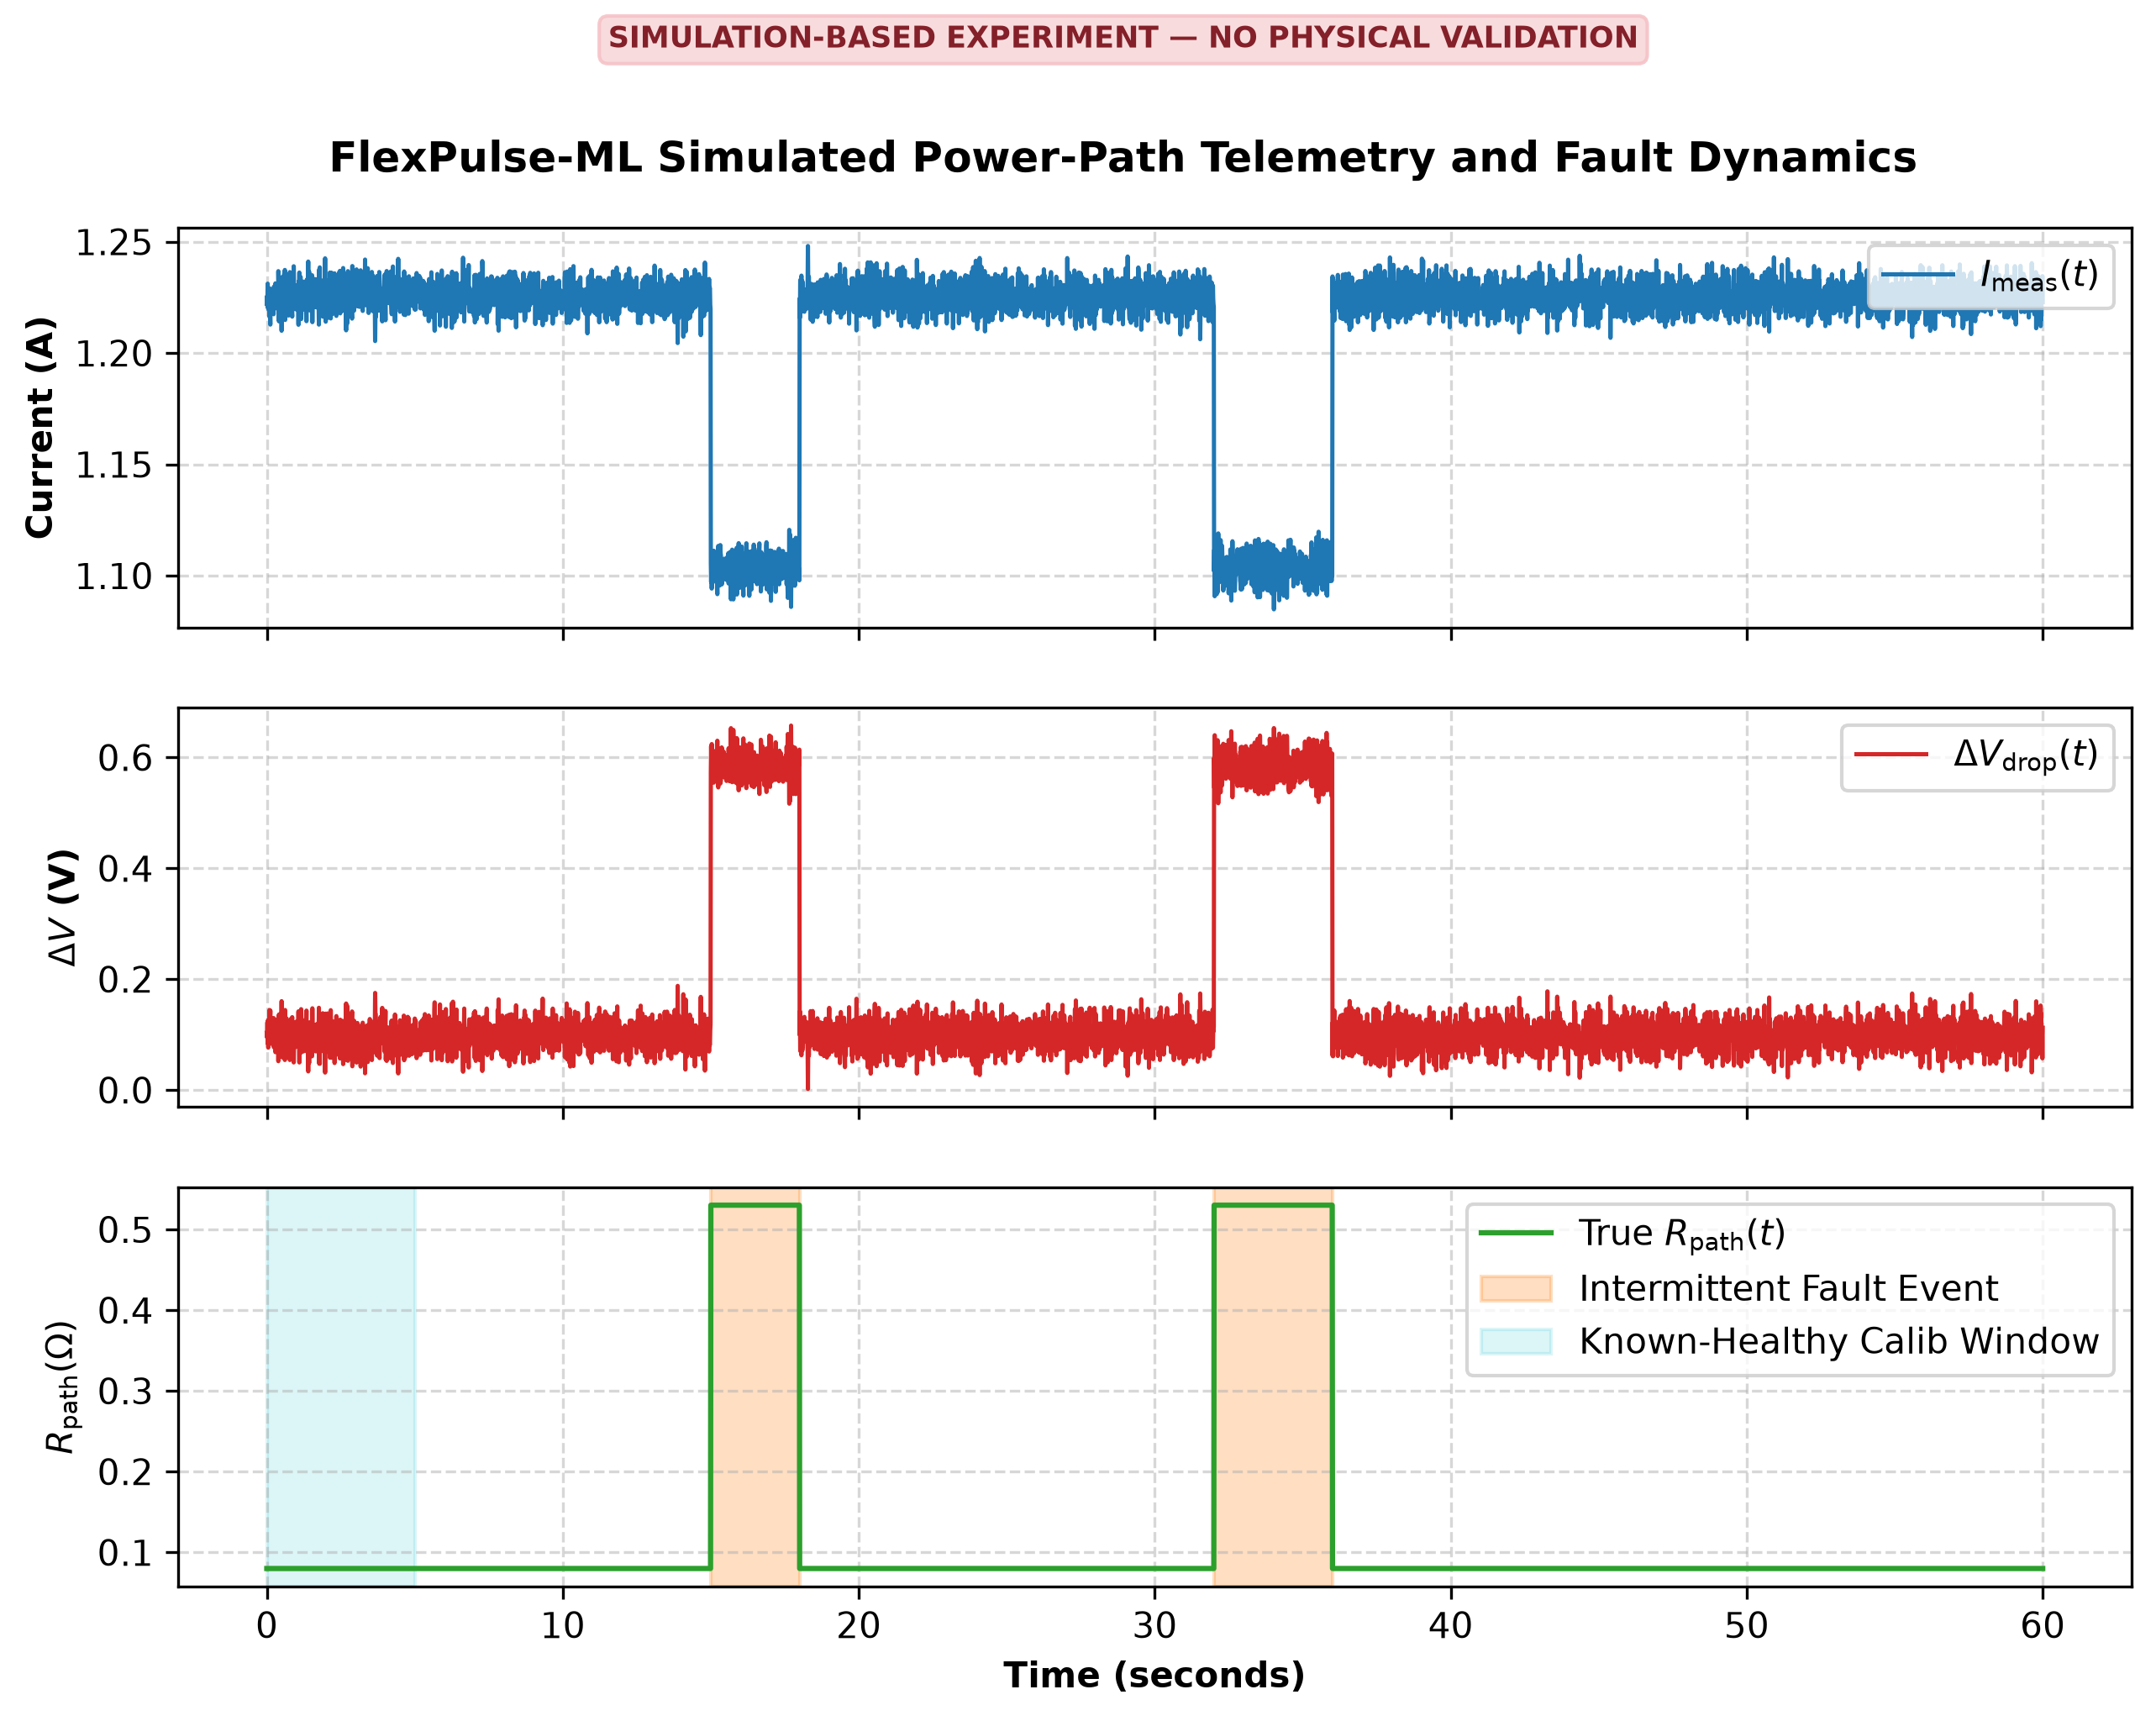
\includegraphics[width=0.85\textwidth,height=5.5cm,keepaspectratio]{figures/fig1_powerpath_architecture_signals.png}
\caption{The FlexPulse-ML research simulation framework. (a) Conceptual DC equivalent circuit showing power supply, total path resistance, load impedance, and terminal sensors. (b) Nine-stage software processing pipeline from simulation to event evaluation. (c) Representative synthetic voltage and current signals under nominal conditions versus shifted out-of-distribution conditions with intermittent contact events.}
\label{fig:framework}
\end{figure*}

\subsection{Circuit Equations}
We model a DC power path delivering electrical power from a source to a load through a separable connector, inspired by a USB-C VBUS/GND circuit path. The electrical circuit is represented by the lumped-parameter equivalent circuit illustrated in Fig.~\ref{fig:framework}(a).

The total instantaneous power-path resistance $R_{\text{path}}(t)$ is defined as:
\begin{equation}
R_{\text{path}}(t) = R_0 + R_{\text{contact}}(t) + R_{\text{fault}}(t)
\label{eq:rpath}
\end{equation}
where $R_0$ is the nominal bulk resistance of the conductor and printed circuit traces, $R_{\text{contact}}(t)$ represents normal mechanical contact interface variations, and $R_{\text{fault}}(t)$ represents abnormal degradation (such as oxidation creep or intermittent contact micro-interruptions).

Applying Ohm's law, the true instantaneous circuit current $I(t)$ and true terminal load voltage $V_{\text{load}}(t)$ are:
\begin{equation}
I(t) = \frac{V_s(t)}{R_{\text{path}}(t) + R_{\text{load}}(t)}
\label{eq:current}
\end{equation}
\begin{equation}
V_{\text{load}}(t) = I(t) \cdot R_{\text{load}}(t) = V_s(t) \cdot \frac{R_{\text{load}}(t)}{R_{\text{path}}(t) + R_{\text{load}}(t)}
\label{eq:voltage}
\end{equation}
where $V_s(t)$ is the source voltage and $R_{\text{load}}(t)$ is the load resistance.

\subsection{Measurement Model and Non-Identifiability}
In an operational system, internal circuit quantities ($R_{\text{path}}$, $V_s$, $R_{\text{load}}$) cannot be observed directly. Instead, telemetry consists solely of sampled voltage and current measurements corrupted by sensor bias and noise:
\begin{equation}
V_{\text{meas}}(t) = V_{\text{load}}(t) + b_V(t) + \eta_V(t)
\label{eq:vmeas}
\end{equation}
\begin{equation}
I_{\text{meas}}(t) = I(t) + b_I(t) + \eta_I(t)
\label{eq:imeas}
\end{equation}
where $b_V(t)$ and $b_I(t)$ are slowly drifting sensor calibration offsets, and $\eta_V(t) \sim \mathcal{N}(0, \sigma_V^2)$ and $\eta_I(t) \sim \mathcal{N}(0, \sigma_I^2)$ represent zero-mean Gaussian measurement noise.

A key theoretical observation is that path resistance $R_{\text{path}}(t)$ is algebraically non-identifiable from terminal measurements alone without prior knowledge of $V_s$ and $R_{\text{load}}$. Calculating an apparent resistance ratio $R_{\text{app}} = V_{\text{meas}} / I_{\text{meas}} \approx R_{\text{load}}$ yields the load resistance, not the path resistance. A voltage drop across the connector produces an observable signature at the load, but a similar drop can be caused by a legitimate decrease in source voltage or an increase in load current. Consequently, simple static thresholding on raw terminal measurements cannot distinguish power-path resistance faults from legitimate load transitions.

\section{Proposed Simulation Framework}
The FlexPulse-ML framework is structured as an end-to-end software pipeline consisting of nine functional stages, shown in Fig.~\ref{fig:framework}(b):
\begin{enumerate}
    \item \textbf{Electrical Equivalent Simulation:} Generates synthetic circuit signals based on (\ref{eq:rpath})--(\ref{eq:voltage}) at a sampling rate of $f_s = 100\,\text{Hz}$ ($0.01\,\text{s}$ time step) for $60\,\text{s}$ runs ($6,000$ points/run).
    \item \textbf{Controlled Fault Injection:} Injects parameterized fault events (intermittent contact jumps, gradual degradation ramps, and slow creeping faults) with exact start and end timestamps.
    \item \textbf{Measurement Degradation:} Applies sensor biases and Gaussian noise according to (\ref{eq:vmeas})--(\ref{eq:imeas}).
    \item \textbf{Sliding-Window Feature Extraction:} Slices signals into overlapping windows of duration $T_w = 0.50\,\text{s}$ (50 samples) with stride $T_s = 0.25\,\text{s}$ (25 samples), producing 239 windows per run.
    \item \textbf{Machine Learning Inference:} Evaluates trained decision models on feature vectors.
    \item \textbf{Initial Reference Calibration:} Uses the initial $5.0\,\text{s}$ guaranteed healthy period to compute a reference baseline and center level features.
    \item \textbf{Defensive Adaptive Updates:} Optionally updates running baselines via Exponential Moving Average (EMA) subject to confidence and stability gating.
    \item \textbf{Temporal Persistence Filtering:} Filters raw binary predictions through a causal $N$-window persistence rule to reject isolated false alarms.
    \item \textbf{Event-Level and Bootstrap Evaluation:} Evaluates detections against ground-truth events and computes paired bootstrap confidence intervals.
\end{enumerate}

\section{Synthetic Dataset and Scenarios}

\subsection{Controlled Scenarios}
To evaluate model robustness under operational shifts, we defined ten distinct operational and fault scenarios, summarized in Table~\ref{tab:scenarios}.

\begin{table}[!t]
\caption{Synthetic Circuit Scenarios in the Confirmatory Evaluation}
\label{tab:scenarios}
\centering
\begingroup
\footnotesize
\setlength{\tabcolsep}{2.8pt}
\begin{tabularx}{\columnwidth}{@{}l>{\raggedright\arraybackslash}p{2.2cm}>{\raggedright\arraybackslash}X@{}}
\toprule
\textbf{ID} & \textbf{Scenario Name} & \textbf{Physical and Electrical Description} \\
\midrule
S1 & Healthy Nominal & Baseline healthy path ($R_0=0.08\,\Omega$, $R_L=4.0\,\Omega$, clean). \\
S2 & Increased Resistance & Elevated path resistance ($R_0=0.22\,\Omega$) + contact jumps. \\
S3 & Intermittent Contact & 3--5 sharp contact disconnects ($\Delta R=0.4$--$0.85\,\Omega$). \\
S4 & Gradual Drift & Linear contact oxidation creep ($+0.003\,\Omega/\text{s}$ after $5\,\text{s}$). \\
S5 & Sensor Offset Drift & Path healthy; linear voltage sensor bias drift ($+2\,\text{mV/s}$). \\
S6 & Noise Shift & 3$\times$ elevated noise ($\sigma_V=0.018\,\text{V}$) + contact events. \\
S7 & Load Operating Shift & Continuous heavy load ($R_L=1.9\,\Omega$, $2.55\,\text{A}$) + contact events. \\
S8 & Abrupt Load Change & Path healthy; load step ($4.0\,\Omega \to 2.0\,\Omega$) at $t=25\,\text{s}$. \\
S9 & Slow Developing Fault & Creeping fault ramp ($0 \to 0.45\,\Omega$ over $25\,\text{s}$). \\
S10 & Combined Shifts & Sensor drift + load step + elevated noise + faults. \\
\bottomrule
\end{tabularx}
\endgroup
\end{table}

\subsection{Dataset Partitions and S4 Ground-Truth Resolution}
\textbf{Model Training Origin:} The underlying machine learning models and threshold envelopes were trained during Phase~5 using the nominal training partition of an earlier dataset, \texttt{flexpulse\_calibration\_v2} (random seed 42, 6 nominal runs, 1,434 sliding windows). The resulting model artifacts (\texttt{a0\_fixed\_threshold.joblib}, \texttt{a1\_static\_random\_forest.joblib}, and \texttt{a2\_a3\_normalized\_random\_forest.joblib}) were frozen in \texttt{models/phase5/}. These frozen artifacts were evaluated prospectively without retraining, parameter re-tuning, or architectural adjustments.

\textbf{Confirmatory Evaluation Dataset:} The confirmatory dataset (\texttt{flexpulse\_final\_test\_v5}) was generated with a separate root random seed (20261202) to evaluate these frozen models. It comprises 82 independent simulation runs (19,598 feature windows):
\begin{itemize}
    \item \textbf{Nominal Reference Partitions:} 6 train runs (1,434 windows) and 6 validation runs (1,434 windows) generated for partition completeness and threshold auditing.
    \item \textbf{In-Distribution (ID) Test Split:} 20 independent runs (4,780 windows; 2 runs per scenario under nominal electrical conditions).
    \item \textbf{Out-of-Distribution (OOD) Test Split:} 50 independent runs (11,950 windows; 5 runs per scenario under shifted operating conditions: elevated noise $\sigma_V=0.015\,\text{V}, \sigma_I=0.022\,\text{A}$, elevated base resistance $R_0=0.140\,\Omega$, sensor biases, and shifted load impedances).
\end{itemize}

\textit{Note on Historical v4 Dataset:} In an earlier test dataset (\texttt{flexpulse\_final\_test\_v4}), Scenario S4 simulated gradual resistance drift by modifying the conductor resistance without setting ground-truth fault flags (\texttt{fault\_labels} = 0). This caused calibrated models that correctly flagged the rising voltage drop to be penalized as false positives. In \texttt{flexpulse\_final\_test\_v5}, S4 is properly labeled as an active electrical fault for $t \ge 5.0\,\text{s}$ ($1,100$ ground-truth positive windows). Because v5 uses an independent seed, results between v4 and v5 are reported transparently as historical versus confirmatory findings, with v5 serving as the primary evidence.

\section{Feature Engineering}
From each $0.50\,\text{s}$ window of measured voltage and current telemetry, we extract 26 observable features (13 from voltage, 13 from current). The features are divided into four mathematical categories:
\begin{enumerate}
    \item \textbf{Level Features (6 per signal):} Mean, median, minimum, maximum, 10th percentile ($p_{10}$), and 90th percentile ($p_{90}$).
    \item \textbf{Spread Features (3 per signal):} Standard deviation, range ($\max - \min$), and median absolute deviation (MAD).
    \item \textbf{Rate Features (1 per signal):} Linear regression slope across the window duration.
    \item \textbf{Differenced Features (3 per signal):} Mean absolute consecutive difference ($\text{mean}(|\Delta x|)$), standard deviation of consecutive differences ($\text{std}(\Delta x)$), and maximum absolute consecutive difference ($\max(|\Delta x|)$).
\end{enumerate}

To implement baseline normalization without corrupting dynamic signatures, level features are centered relative to the estimated baseline ($\tilde{V} = V - \hat{V}_0$, $\tilde{I} = I - \hat{I}_0$). Spread, rate, and differenced features represent intrinsic high-frequency variability and slopes; subtracting a constant level offset from these features is mathematically redundant and physically unjustified. Therefore, spread and rate features remain uncentered.

\section{Machine Learning Detection Architectures}
During Phase~4 exploratory benchmarking, multiple standard classifiers (Logistic Regression, Decision Trees, Random Forests, Support Vector Machines, and Gradient Boosting) were evaluated on nominal telemetry. Random Forest demonstrated the highest empirical stability and was chosen as the primary classification engine.

In Random Forest inference, the model output represents an empirical tree-vote fraction:
\begin{equation}
s(y=c) = \frac{1}{M} \sum_{m=1}^M \mathbb{I}(h_m(\mathbf{x}) = c)
\label{eq:rf_score}
\end{equation}
where $M=100$ is the number of decision trees and $h_m(\mathbf{x})$ is the binary prediction of the $m$-th tree. Because formal probability calibration (such as Platt scaling or isotonic regression) was not independently fitted, $s(y=c)$ is interpreted as an uncalibrated model confidence score or vote fraction rather than a true posterior probability. For binary alert generation, standard majority voting ($\tau = 0.5$) is applied.

For the final evaluation, we examine six standardized detection configurations:
\begin{itemize}
    \item \textbf{M1 (A0) --- Fixed Threshold Baseline:} Predicts a fault when raw observed voltage or current exceeds $\mu_{\text{train}} \pm 2.5\sigma_{\text{train}}$.
    \item \textbf{M2 (A1) --- Static Random Forest:} 100 decision trees (maximum depth 8) trained on raw unnormalized 26-feature vectors from nominal training telemetry.
    \item \textbf{M3 (A2) --- Initial Reference Calibration:} Features normalized relative to the initial $5.0\,\text{s}$ healthy baseline, evaluated with a Random Forest trained on normalized nominal features.
    \item \textbf{M4 (A3) --- Confidence-Gated Adaptive Calibration:} Normalized Random Forest with online baseline updates governed by multi-stage safety gates.
    \item \textbf{M5 (A2+P) --- Initial Calibration + Persistence ($N=2$):} Architecture M3 augmented with a causal two-window persistence filter.
    \item \textbf{M6 (A3+P) --- Adaptive Calibration + Persistence ($N=2$):} Architecture M4 augmented with a causal two-window persistence filter.
\end{itemize}

\section{Reference Calibration and Defensive Adaptive Updates}

\subsection{Initial Reference Calibration}
In practical applications, electrical systems often experience a brief known-healthy state immediately following connection or power-up before physical degradation accelerates. FlexPulse-ML utilizes an initial $5.0\,\text{s}$ reference window ($0.0 \le t \le 5.0\,\text{s}$, 19 feature windows) to estimate the baseline voltage $\hat{V}_0$ and current $\hat{I}_0$:
\begin{equation}
\hat{V}_0 = \text{median}(\{V_{\text{mean}, k}\}_{k=1}^{19}), \quad \hat{I}_0 = \text{median}(\{I_{\text{mean}, k}\}_{k=1}^{19})
\label{eq:calib}
\end{equation}
Subsequent level features are centered by subtracting these estimated initial operating levels.

\subsection{Defensive Adaptive Updates and Safety Gates}
In configuration M4, the baseline is permitted to adapt online via an Exponential Moving Average (EMA) with learning rate $\alpha = 0.04$:
\begin{equation}
\hat{V}_{k} = (1 - \alpha)\hat{V}_{k-1} + \alpha V_{\text{mean}, k}
\label{eq:ema}
\end{equation}

To prevent the baseline estimator from absorbing slow-developing faults, updates are admitted only when all of the following six safety conditions are satisfied:
\begin{enumerate}
    \item \textbf{Initialization Exemption:} The sliding window index exceeds the initial $5.0\,\text{s}$ calibration interval ($k > 19$).
    \item \textbf{Model Confidence Gate:} The tree-vote confidence score for healthy operation satisfies $s(y=0) \ge \tau_{\text{conf}} = 0.95$.
    \item \textbf{Current Stability Gate:} The window current standard deviation $\sigma_I$ (extracted from feature \texttt{current\_std\_a}, defined in configuration by parameter \texttt{max\_current\_variance} = $0.015$) satisfies $\sigma_I \le 0.015\,\text{A}$ (equivalent to current variance $\sigma_I^2 \le 2.25 \times 10^{-4}\,\text{A}^2$), inhibiting updates during load transitions and elevated current jitter.
    \item \textbf{Step Size Bound:} Incremental baseline change satisfies $|\Delta \hat{V}| \le 0.030\,\text{V}$.
    \item \textbf{Outlier Multiplier Check:} Residual error does not exceed $2.5\times$ the initial reference standard deviation.
    \item \textbf{Cooldown and Recovery Logic:} No anomaly has been flagged within the preceding 4 windows, and stable conditions have persisted for at least 5 consecutive windows.
\end{enumerate}

\section{Temporal Persistence Filtering}
Intermittent electrical noise spikes and sensor jitter often cause isolated single-window false detections. To reject these transient false alarms, we implement a causal multi-window persistence filter. For persistence length $N=2$, the filter outputs a positive fault alert at window $k$ if and only if the raw classifier predicted a fault for two consecutive windows:
\begin{equation}
\hat{y}_{\text{filt}, k} = \prod_{j=0}^{N-1} \hat{y}_{\text{raw}, k-j}
\label{eq:persistence}
\end{equation}
Because the stride between successive windows is $T_s = 0.25\,\text{s}$, a two-window filter requires confirmation across $0.25\,\text{s}$, introducing a theoretical minimum causal latency of $+0.25\,\text{s}$ for fault detection.

\section{Experimental Protocol and Evaluation Metrics}
All models, hyperparameters, and feature extraction settings were frozen prior to evaluating the confirmatory dataset. We evaluate performance at two distinct levels:
\begin{itemize}
    \item \textbf{Window-Level Classification:} Evaluated across all 239 windows per run using Accuracy, Balanced Accuracy, Precision, Recall, Specificity, and F1-score.
    \item \textbf{Event-Level Fault Detection:} An injected fault event is scored as \textit{detected} if at least one positive prediction occurs while the fault is active. We report Event Recall ($N_{\text{detected}} / N_{\text{total}}$), the count of False Alarm events during healthy periods, False Alarm rate per minute of healthy operation (FA/min), and causal detection latency ($\tau_{\text{first}} - \tau_{\text{onset}}$).
\end{itemize}

To evaluate statistical significance without violating independence assumptions through overlapping windows, we employ a \textbf{paired run-level bootstrap}~\cite{efron1993introduction} ($B = 1,000$ resamples) clustered at the simulation run level ($N=50$ OOD runs). We compute 95\% empirical bootstrap confidence intervals and two-sided empirical $p$-values.

\section{Results}

\subsection{Overall ID and OOD Comparative Performance}
Table~\ref{tab:overall_perf} presents the primary benchmark results on both the In-Distribution (ID) and Out-of-Distribution (OOD) test sets. Fig.~\ref{fig:id_vs_ood} provides a visual comparison of F1-scores and balanced accuracies.

\begin{table*}[!t]
\caption{Overall Performance Benchmark on Confirmatory Test Dataset (\texttt{flexpulse\_final\_test\_v5})}
\label{tab:overall_perf}
\centering
\begingroup
\footnotesize
\setlength{\tabcolsep}{3.8pt}
\begin{tabular*}{\textwidth}{@{\extracolsep{\fill}}llccccccccc@{}}
\toprule
\textbf{ID} & \textbf{Detection Architecture} & \textbf{Accuracy} & \textbf{Bal. Acc.} & \textbf{Precision} & \textbf{Recall} & \textbf{Specificity} & \textbf{F1-Score} & \textbf{Event Rec.} & \textbf{FA/min} & \textbf{Delay (s)} \\
\midrule
\multicolumn{11}{l}{\textit{In-Distribution (ID) Partition ($N=20$ runs, 4,780 sliding windows)}} \\
\midrule
M1 & Fixed Threshold Envelope (A0) & 0.8395 & 0.7730 & 0.6123 & 0.6578 & 0.8883 & 0.6342 & 100.0\% & 1.88 & 0.1196 \\
M2 & Static Random Forest (A1) & 0.8858 & 0.8545 & 0.7016 & 0.8002 & 0.9087 & 0.7477 & 76.00\% & 0.00 & 0.1196 \\
M3 & Initial Ref. Calibration (A2) & 0.9780 & 0.9687 & 0.9441 & 0.9525 & 0.9849 & 0.9483 & 92.00\% & 1.69 & 0.1196 \\
M4 & Confidence-Gated Adaptive (A3) & 0.9778 & 0.9682 & 0.9441 & 0.9515 & 0.9849 & 0.9478 & 92.00\% & 1.69 & 0.1196 \\
M5 & Initial Calib. + Persistence $N=2$ & 0.9805 & 0.9623 & 0.9761 & 0.9308 & 0.9939 & 0.9529 & 92.00\% & 0.56 & 0.3696 \\
M6 & Adaptive + Persistence $N=2$ & 0.9803 & 0.9618 & 0.9761 & 0.9298 & 0.9939 & 0.9524 & 92.00\% & 0.56 & 0.3696 \\
\midrule
\multicolumn{11}{l}{\textit{Out-of-Distribution (OOD) Partition ($N=50$ runs, 11,950 sliding windows)}} \\
\midrule
M1 & Fixed Threshold Envelope (A0) & 0.4165 & 0.5725 & 0.2488 & 0.8465 & 0.2984 & 0.3846 & 100.0\% & 9.00 & 0.1239 \\
M2 & Static Random Forest (A1) & 0.8664 & 0.8115 & 0.6810 & 0.7148 & 0.9081 & 0.6975 & 76.56\% & 0.05 & 0.1322 \\
M3 & Initial Ref. Calibration (A2) & 0.8722 & 0.9028 & 0.6350 & 0.9565 & 0.8491 & 0.7633 & 92.19\% & 12.95 & 0.1322 \\
M4 & Confidence-Gated Adaptive (A3) & 0.8722 & 0.9028 & 0.6350 & 0.9565 & 0.8491 & 0.7633 & 92.19\% & 12.95 & 0.1322 \\
M5 & Initial Calib. + Persistence $N=2$ & \textbf{0.9321} & \textbf{0.9335} & \textbf{0.7885} & 0.9359 & \textbf{0.9311} & \textbf{0.8559} & 92.19\% & 7.92 & 0.3407 \\
M6 & Adaptive + Persistence $N=2$ & \textbf{0.9321} & \textbf{0.9335} & \textbf{0.7885} & 0.9359 & \textbf{0.9311} & \textbf{0.8559} & 92.19\% & 7.92 & 0.3407 \\
\bottomrule
\end{tabular*}
\endgroup
\end{table*}

\begin{figure}[!t]
\centering
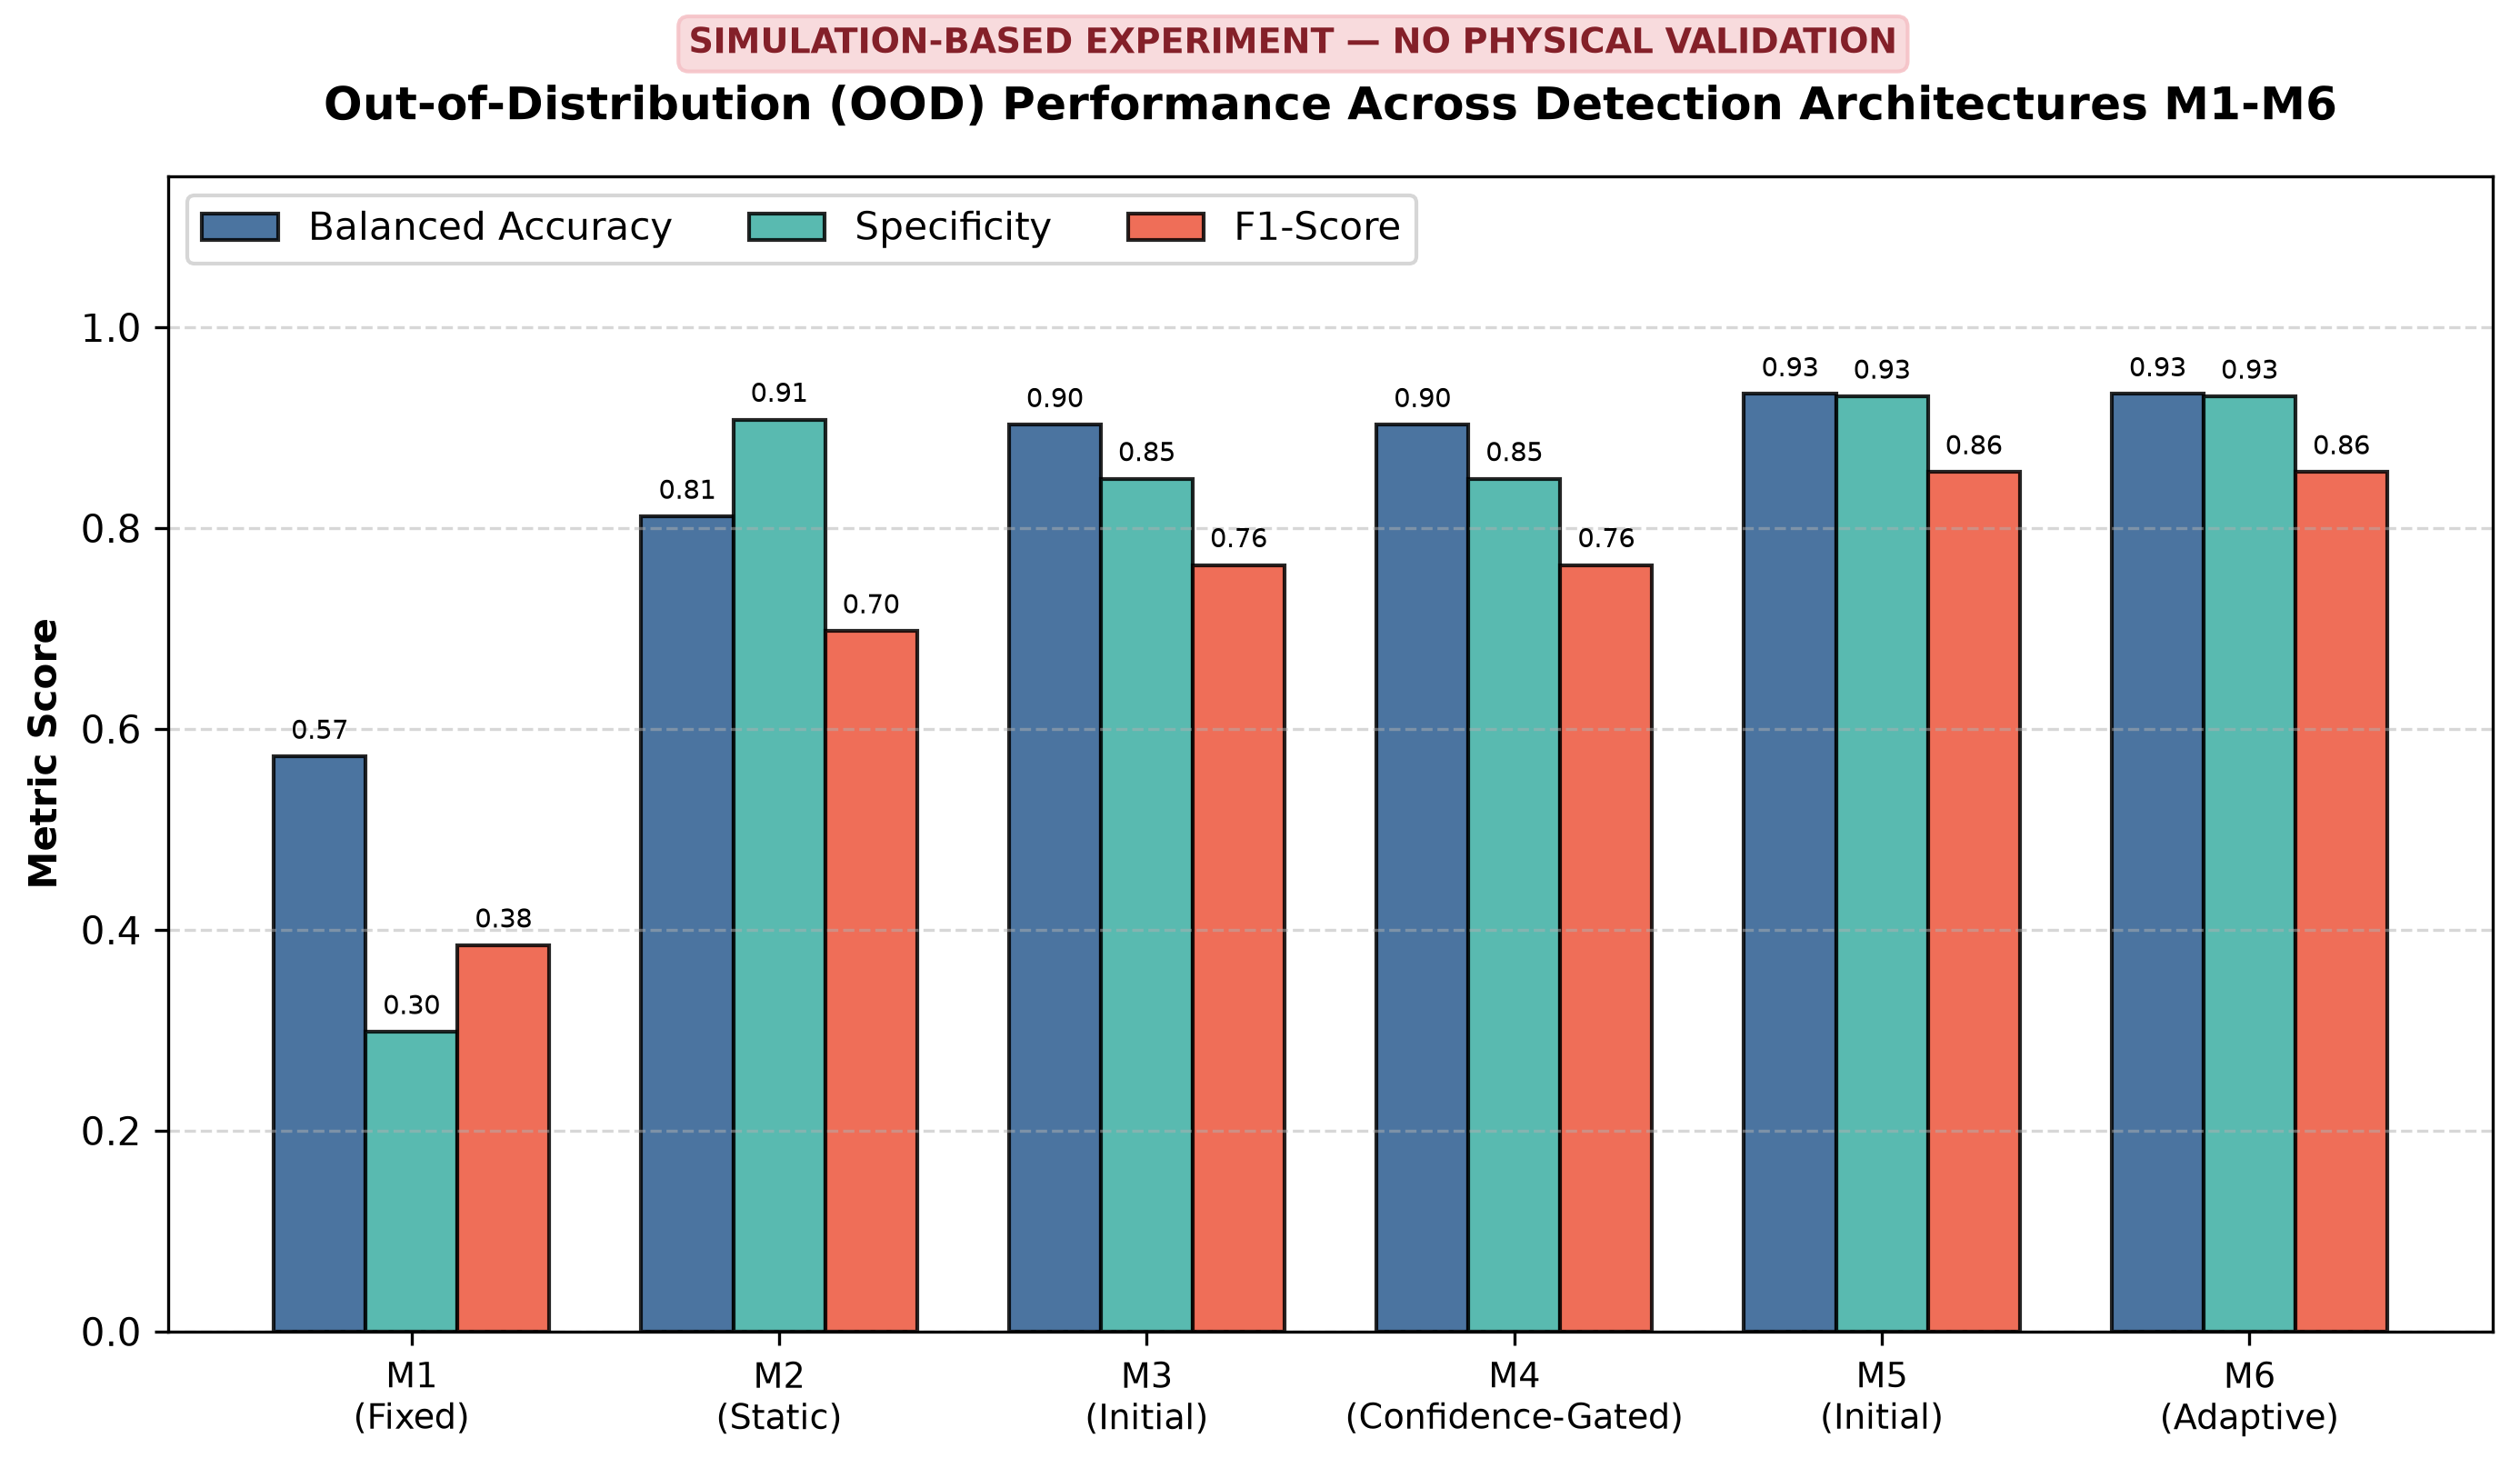
\includegraphics[width=0.92\columnwidth]{figures/fig2_id_vs_ood_comparative_performance.png}
\caption{In-Distribution (ID) versus Out-of-Distribution (OOD) comparative performance across methods. While static Random Forest (M2) degrades significantly under OOD shifts, initial calibration with persistence (M5) maintains high balanced accuracy (0.9335) and F1-score (0.8559).}
\label{fig:id_vs_ood}
\end{figure}

On OOD test runs, Fixed Threshold (M1) suffers severe degradation: specificity collapses to 0.2984, resulting in an OOD F1-score of 0.3846 and 9.00 false alarms per minute. Static Random Forest (M2) maintains high specificity (0.9081) but exhibits inadequate fault sensitivity, missing 15 of 64 OOD fault events (Event Recall = 76.56\%, window recall = 0.7148). 

Initial reference calibration (M3) restores fault sensitivity across shifted regimes, achieving a window recall of 0.9565 and event recall of 92.19\% (59 of 64 events detected). However, elevated sensitivity increases raw false alarms under noise (12.95 FA/min), limiting its raw F1-score to 0.7633. 

Adding causal two-window persistence filtering (M5) resolves this trade-off: false alarms drop from 12.95 to 7.92 FA/min, specificity rises from 0.8491 to 0.9311, and F1-score increases to \textbf{0.8559}, while retaining 100\% of the fault events detected by M3 (59 of 64 events).

\subsection{Bootstrap Significance and Equivalence Testing}
Table~\ref{tab:bootstrap} reports the paired run-level bootstrap hypothesis tests ($B=1,000$).

\begin{table*}[!t]
\caption{Paired Run-Level Bootstrap Significance ($B=1,000$ Iterations on OOD Partition)}
\label{tab:bootstrap}
\centering
\begingroup
\footnotesize
\setlength{\tabcolsep}{3.5pt}
\begin{tabularx}{\textwidth}{@{}lp{3.2cm}ccccc>{\raggedright\arraybackslash}X@{}}
\toprule
\textbf{Comparison} & \textbf{Hypothesis Tested} & $\mathbf{\Delta}$\textbf{F1 (Mean)} & \textbf{95\% CI F1} & $\mathbf{\Delta}$\textbf{BalAcc} & \textbf{95\% CI BalAcc} & \textbf{Empirical} $p$ & \textbf{Empirical Scientific Verdict} \\
\midrule
M2 vs M1 & Static ML vs. Fixed Baseline & $+0.3169$ & $[+0.2084, +0.4322]$ & $+0.2384$ & $[+0.1888, +0.2865]$ & $< 0.01$ & Significant F1 gain; static ML avoids threshold collapse. \\
M3 vs M2 & Initial Calib. vs. Static ML & $+0.0595$ & $[-0.0648, +0.1596]$ & $+0.0896$ & $[+0.0398, +0.1379]$ & $0.3220$ & Significant BalAcc gain ($p<0.01$); F1 CI spans zero due to raw FAs. \\
M4 vs M3 & Adaptive Calib. vs. Initial Calib. & $0.0000$ & $[0.0000, 0.0000]$ & $0.0000$ & $[0.0000, 0.0000]$ & $1.0000$ & Statistically identical; zero incremental adaptive benefit. \\
M5 vs M3 & Persistence vs. Raw Initial Calib. & $+0.0932$ & $[+0.0684, +0.1223]$ & $+0.0304$ & $[+0.0224, +0.0382]$ & $< 0.01$ & Statistically significant; persistence suppresses noise FAs. \\
M6 vs M4 & Persistence vs. Raw Adaptive Calib. & $+0.0932$ & $[+0.0684, +0.1223]$ & $+0.0304$ & $[+0.0224, +0.0382]$ & $< 0.01$ & Statistically significant; persistence suppresses noise FAs. \\
\bottomrule
\end{tabularx}
\endgroup
\end{table*}

The paired bootstrap comparison between M4 (adaptive calibration) and M3 (initial calibration) yields $\Delta\text{F1} = 0.0000$ across all 1,000 bootstrap resamples ($p = 1.0000$) on the OOD evaluation partition. On these 50 OOD test runs (11,950 sliding windows), defensive safety gates remained active during anomalous intervals, causing M4 to generate classifications identical to M3. On in-distribution test runs, a minor single-window divergence occurs (ID F1 of 0.9483 for M3 vs 0.9478 for M4). Thus, continuous adaptive updates provided zero incremental benefit over initial reference calibration under shifted operating conditions. Conversely, persistence filtering (M5 vs M3) produces a statistically significant improvement ($\Delta\text{F1} = +0.0932$, 95\% CI $[+0.0684, +0.1223]$, $p < 0.01$).

\subsection{Scenario-Specific Breakdown and Failure Modes}
Table~\ref{tab:scenario_breakdown} and Fig.~\ref{fig:scenarios} detail model performance across all ten scenarios.

\begin{figure*}[!t]
\centering
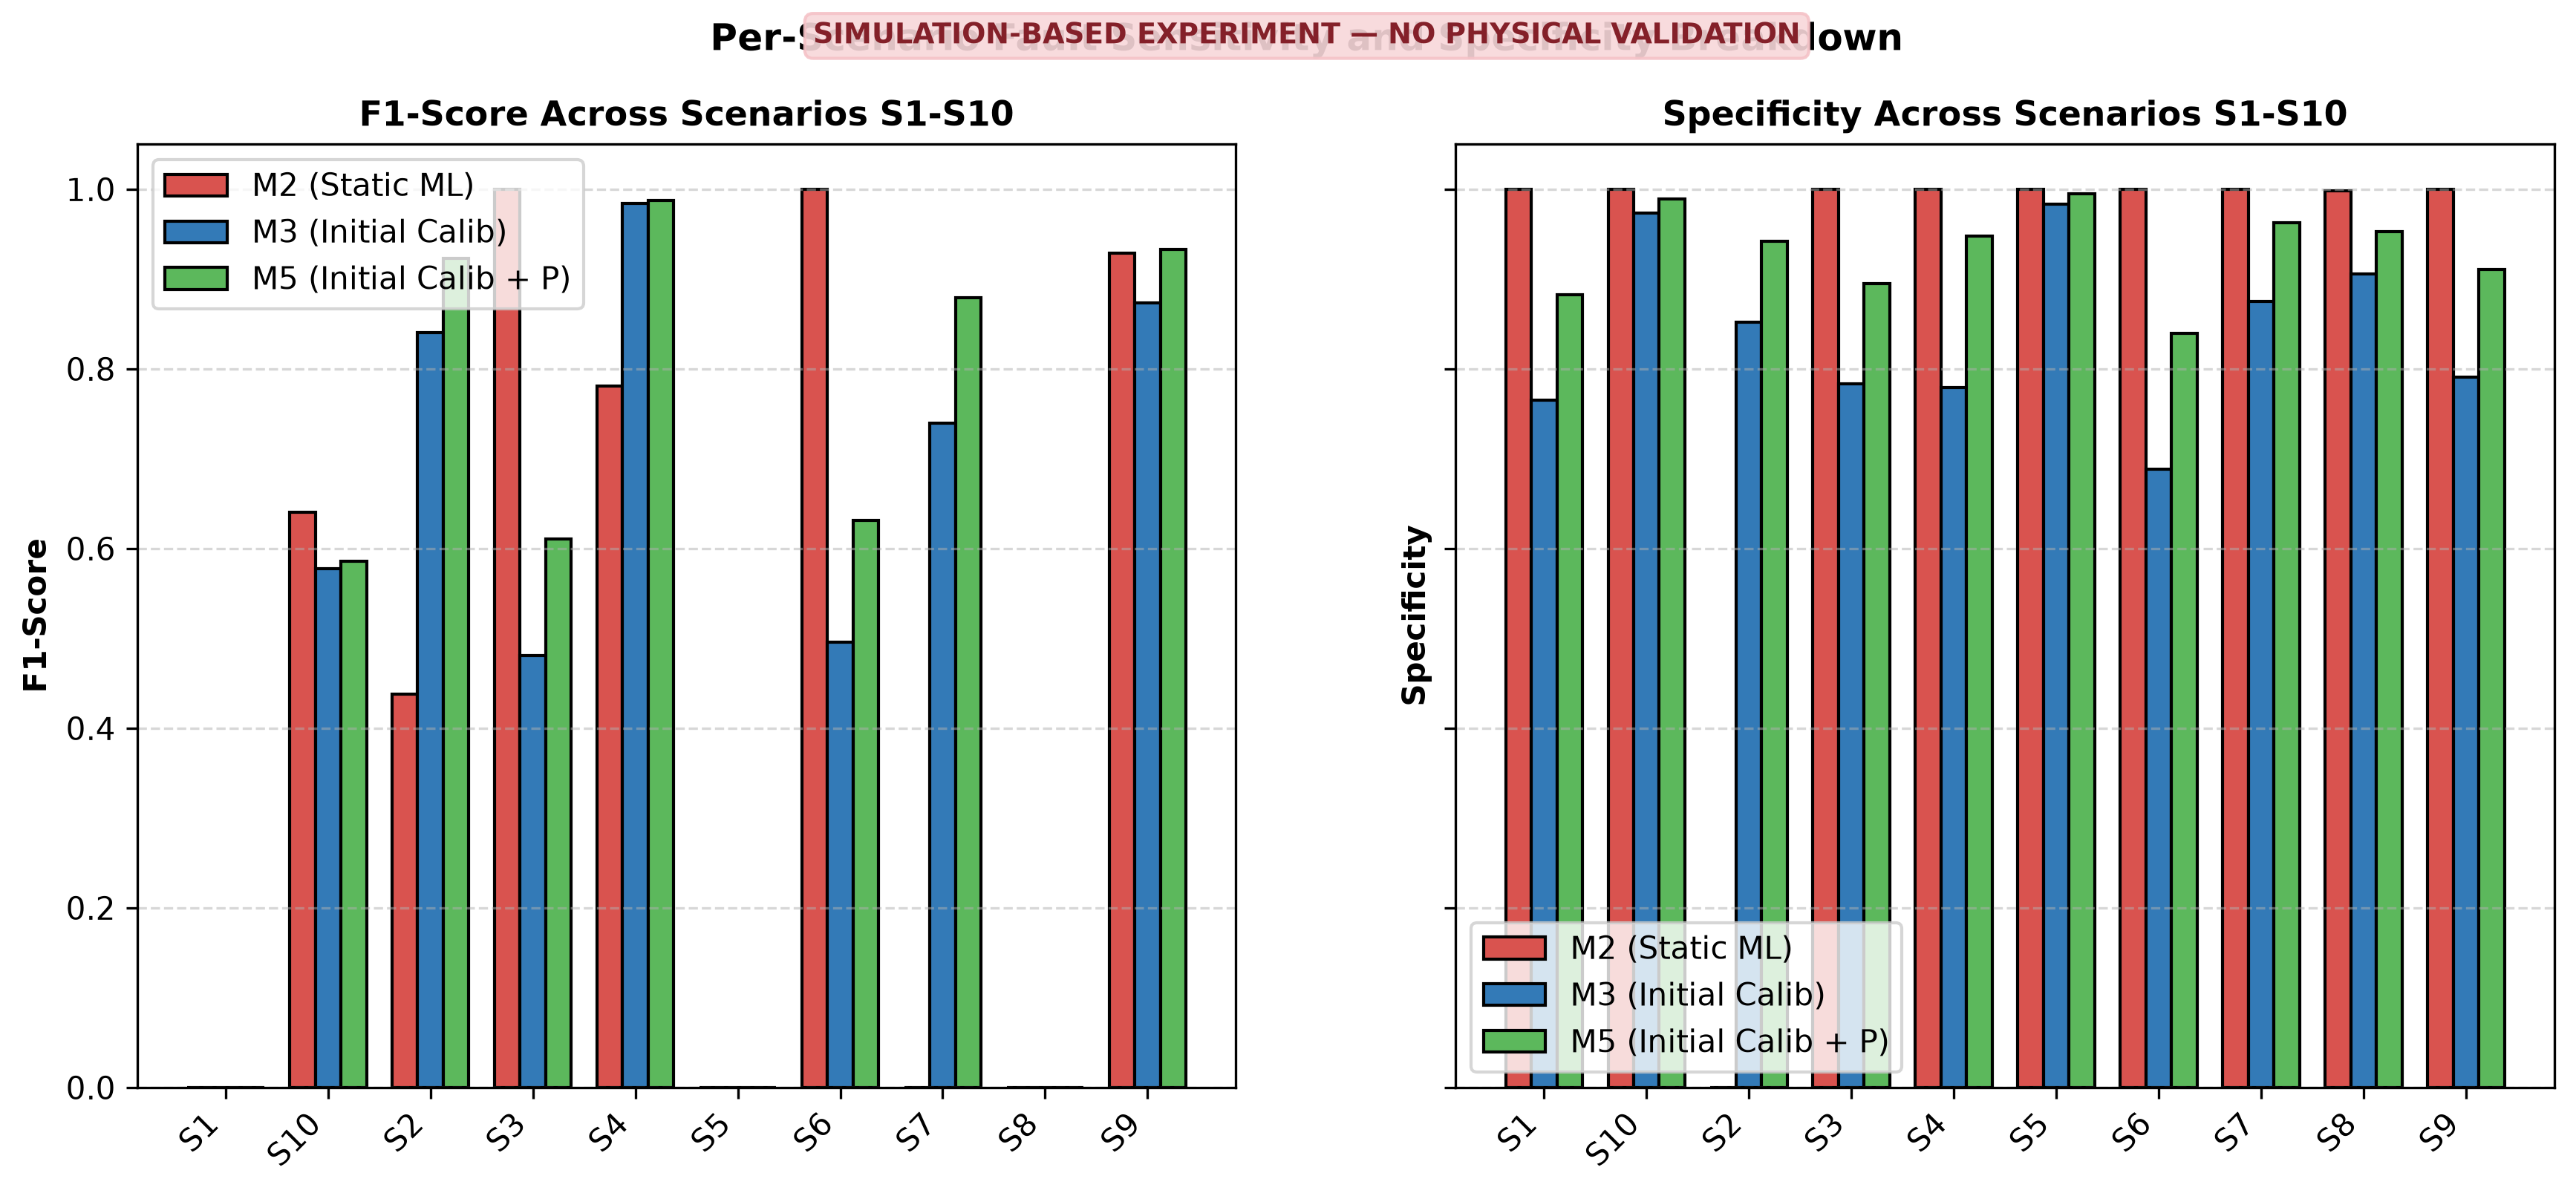
\includegraphics[width=0.85\textwidth,height=5.2cm,keepaspectratio]{figures/fig3_scenario_breakdown.png}
\caption{Detailed scenario-by-scenario performance across all ten controlled physical regimes in the OOD test set, demonstrating the catastrophic failure of static ML (M2) on S7 (heavy load) and S2 (elevated resistance), and the restoration of performance by M3 and M5.}
\label{fig:scenarios}
\end{figure*}

\begin{table}[!t]
\caption{Scenario-Specific Performance Breakdown in OOD Test Set}
\label{tab:scenario_breakdown}
\centering
\begingroup
\footnotesize
\setlength{\tabcolsep}{2.0pt}
\begin{tabular*}{\columnwidth}{@{\extracolsep{\fill}}llcccc@{}}
\toprule
\textbf{Scenario} & \textbf{ID} & \textbf{Pos} & \textbf{Recall} & \textbf{Spec.} & \textbf{F1} \\
\midrule
S1: Nominal           & M1 & 0    & N/A    & 0.3289 & N/A \\
                      & M2 & 0    & N/A    & 1.0000 & N/A \\
                      & M3 & 0    & N/A    & 0.7649 & N/A \\
                      & M5 & 0    & N/A    & 0.8828 & N/A \\
\midrule
S2: Elevated $R_0$    & M1 & 335  & 1.0000 & 0.3500 & 0.5452 \\
                      & M2 & 335  & 1.0000 & \textbf{0.0000} & 0.4379 \\
                      & M3 & 335  & 1.0000 & 0.8523 & 0.8407 \\
                      & M5 & 335  & 0.9851 & \textbf{0.9419} & \textbf{0.9231} \\
\midrule
S4: Gradual Drift     & M1 & 1100 & 0.6982 & 0.3684 & 0.7967 \\
                      & M2 & 1100 & 0.6409 & 1.0000 & 0.7812 \\
                      & M3 & 1100 & \textbf{0.9873} & 0.7789 & \textbf{0.9841} \\
                      & M5 & 1100 & \textbf{0.9791} & \textbf{0.9474} & \textbf{0.9872} \\
\midrule
S7: Load Shift        & M1 & 180  & 1.0000 & 0.3419 & 0.3502 \\
                      & M2 & 180  & \textbf{0.0000} & 1.0000 & \textbf{0.0000} \\
                      & M3 & 180  & 1.0000 & 0.8749 & 0.7392 \\
                      & M5 & 180  & 0.9500 & 0.9626 & \textbf{0.8792} \\
\midrule
S8: Load Step         & M1 & 0    & N/A    & 0.3423 & N/A \\
                      & M2 & 0    & N/A    & 0.9983 & N/A \\
                      & M3 & 0    & N/A    & 0.9054 & N/A \\
                      & M5 & 0    & N/A    & 0.9531 & N/A \\
\midrule
S9: Slow Creep        & M1 & 521  & 0.8791 & 0.3234 & 0.6383 \\
                      & M2 & 521  & 0.8676 & 1.0000 & 0.9291 \\
                      & M3 & 521  & 0.9846 & 0.7908 & 0.8732 \\
                      & M5 & 521  & 0.9750 & 0.9110 & 0.9330 \\
\bottomrule
\end{tabular*}
\endgroup
\end{table}

This breakdown exposes two critical failure modes of Static Random Forest (M2):
\begin{enumerate}
    \item \textbf{Complete Sensitivity Collapse on Load Shift (S7):} Under continuous heavy load ($R_{\text{load}} = 1.9\,\Omega, I \approx 2.55\,\text{A}$), M2 failed to detect a single fault window (Recall = 0.0000, F1 = 0.0000). Because nominal training data contained only 1.25\,A operating points, the model misclassified the altered operating region entirely. In contrast, M3 achieved 1.0000 recall (F1 = 0.7392), and M5 achieved 0.9500 recall (F1 = 0.8792).
    \item \textbf{Specificity Collapse on Elevated Conductor Resistance (S2):} When baseline conductor resistance was elevated to $R_0 = 0.220\,\Omega$, M2 produced 860 false-positive windows (Specificity = 0.0000). Reference calibration normalized this static offset, restoring specificity to 0.8523 (M3) and 0.9419 (M5).
    \item \textbf{Gradual Resistance Drift (S4):} Static RF missed 35.91\% of S4 gradual drift windows (Recall = 0.6409). M3 detected 98.73\% of degradation windows (F1 = 0.9841), and M5 detected 97.91\% (F1 = 0.9872).
\end{enumerate}

\subsection{Temporal Persistence Ablation}
Table~\ref{tab:persistence} and Fig.~\ref{fig:persistence} illustrate the trade-off as persistence length $N$ increases from 1 to 5.

\begin{figure}[!t]
\centering
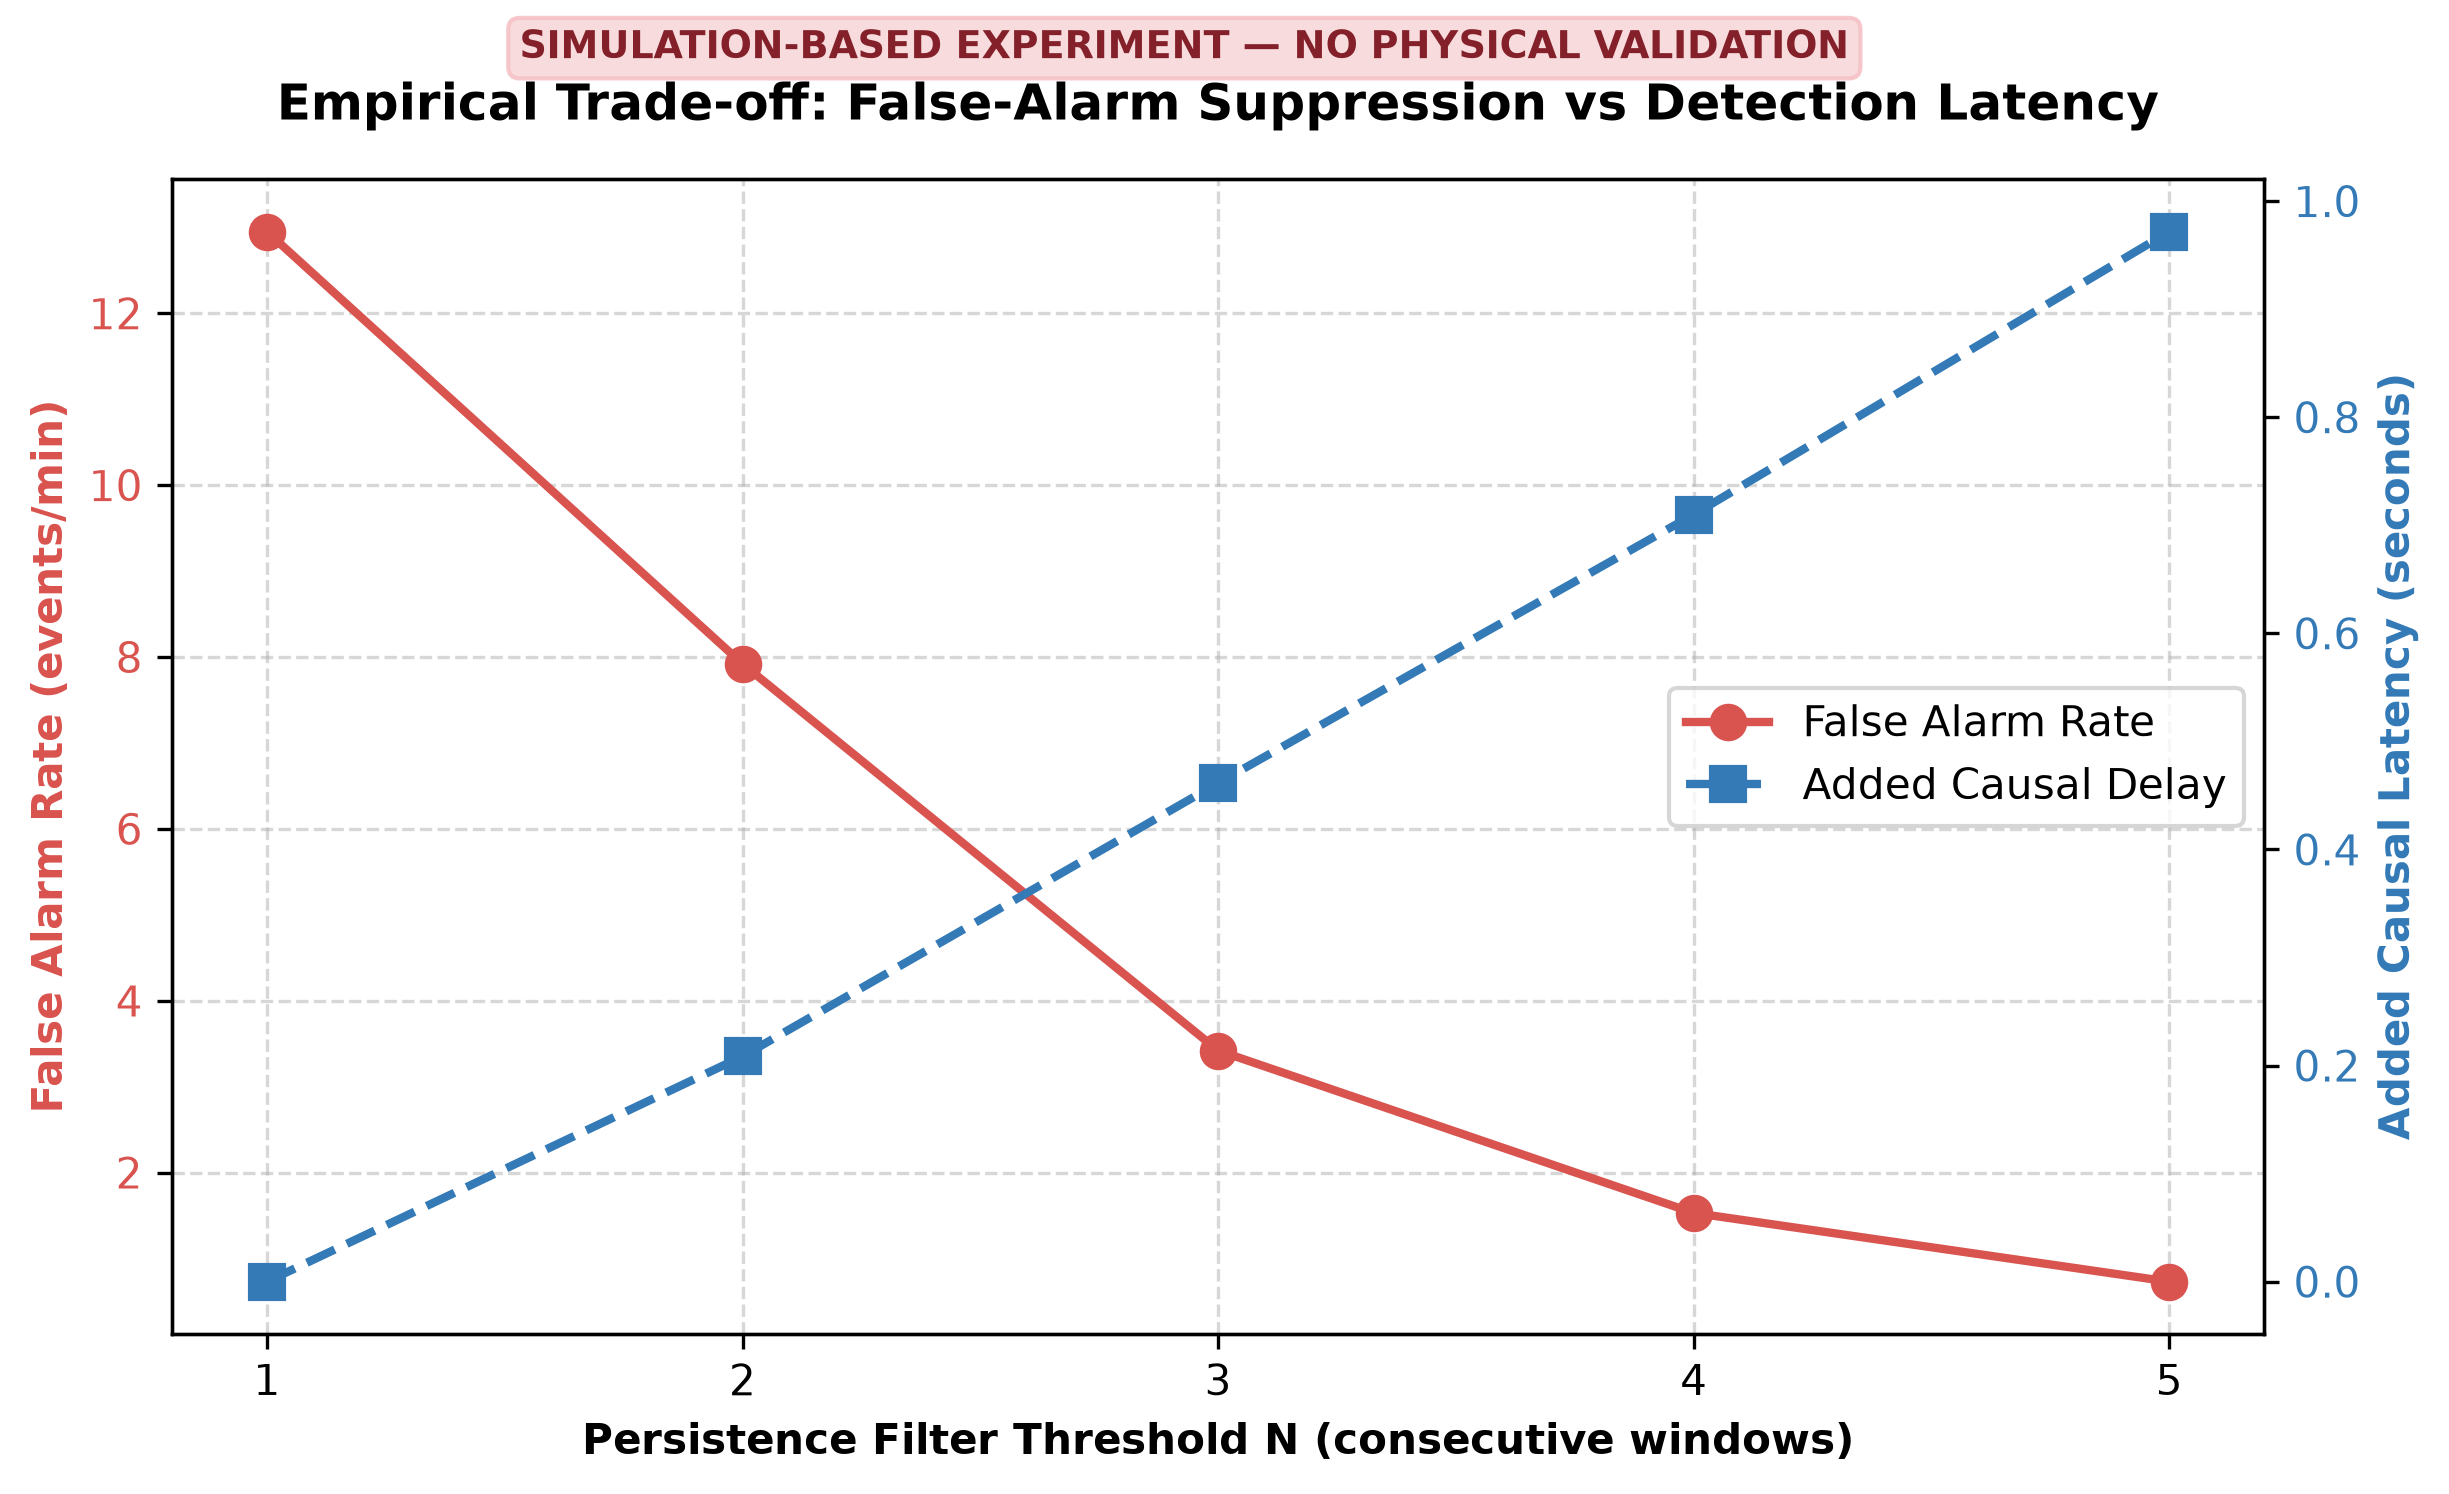
\includegraphics[width=0.92\columnwidth]{figures/fig4_persistence_tradeoff_curve.png}
\caption{Temporal persistence filter trade-off curve across filter lengths $N \in \{1, 2, 3, 4, 5\}$. Length $N=2$ provides substantial false-alarm reduction (38.83\%) with zero event recall loss, while $N \ge 4$ causes fault events to be missed.}
\label{fig:persistence}
\end{figure}

\begin{table}[!t]
\caption{Temporal Persistence Ablation on OOD Test Split}
\label{tab:persistence}
\centering
\begingroup
\footnotesize
\setlength{\tabcolsep}{2.5pt}
\begin{tabular*}{\columnwidth}{@{\extracolsep{\fill}}ccccccc@{}}
\toprule
$N$ & \textbf{Acc.} & \textbf{F1} & \textbf{Spec.} & \textbf{Ev. Rec.} & \textbf{FA Red.} & \textbf{Added Delay} \\
\midrule
1 & 0.8722 & 0.7633 & 0.8491 & 92.19\% & 0.00\% & $0.0000\,\text{s}$ \\
\textbf{2} & \textbf{0.9321} & \textbf{0.8559} & \textbf{0.9311} & \textbf{92.19\%} & \textbf{38.83\%} & $\mathbf{+0.2085\,\text{s}}$ \\
3 & 0.9582 & 0.9039 & 0.9703 & 92.19\% & 73.59\% & $+0.4614\,\text{s}$ \\
4 & 0.9649 & 0.9163 & 0.9852 & 90.62\% & 88.16\% & $+0.7099\,\text{s}$ \\
5 & 0.9652 & 0.9149 & 0.9918 & 85.94\% & 94.37\% & $+0.9717\,\text{s}$ \\
\bottomrule
\end{tabular*}
\endgroup
\end{table}

While window-level F1-score continues to rise for $N=3$ (0.9039) and $N=4$ (0.9163) due to continued suppression of false-positive windows, longer persistence filters introduce substantial latency penalties: median detection delay increases by $+0.4614\,\text{s}$ for $N=3$ (total delay $0.5936\,\text{s}$) and $+0.7099\,\text{s}$ for $N=4$ (total delay $0.8421\,\text{s}$). Crucially, when $N \ge 4$, short intermittent micro-interruptions are filtered out, causing Event Recall to degrade to 90.62\% at $N=4$ (missing 6 events) and 85.94\% at $N=5$ (missing 9 events). 

Filter length $N=2$ was therefore selected not as a universally optimal parameter, but as an effective lower-latency engineering compromise: it reduces false-alarm events by 38.83\% ($515 \to 315$) while maintaining 100\% of the fault events detected by raw calibration (Event Recall remains 92.19\%, 59 of 64 events) at an added median latency of $+0.2085\,\text{s}$ (total median delay $0.3407\,\text{s}$).

\subsection{Gating Integrity and Tracker Contamination}
Table~\ref{tab:gating} and Fig.~\ref{fig:gating} evaluate gating performance on Scenario S9 (Slow Developing Fault).

\begin{figure}[!t]
\centering
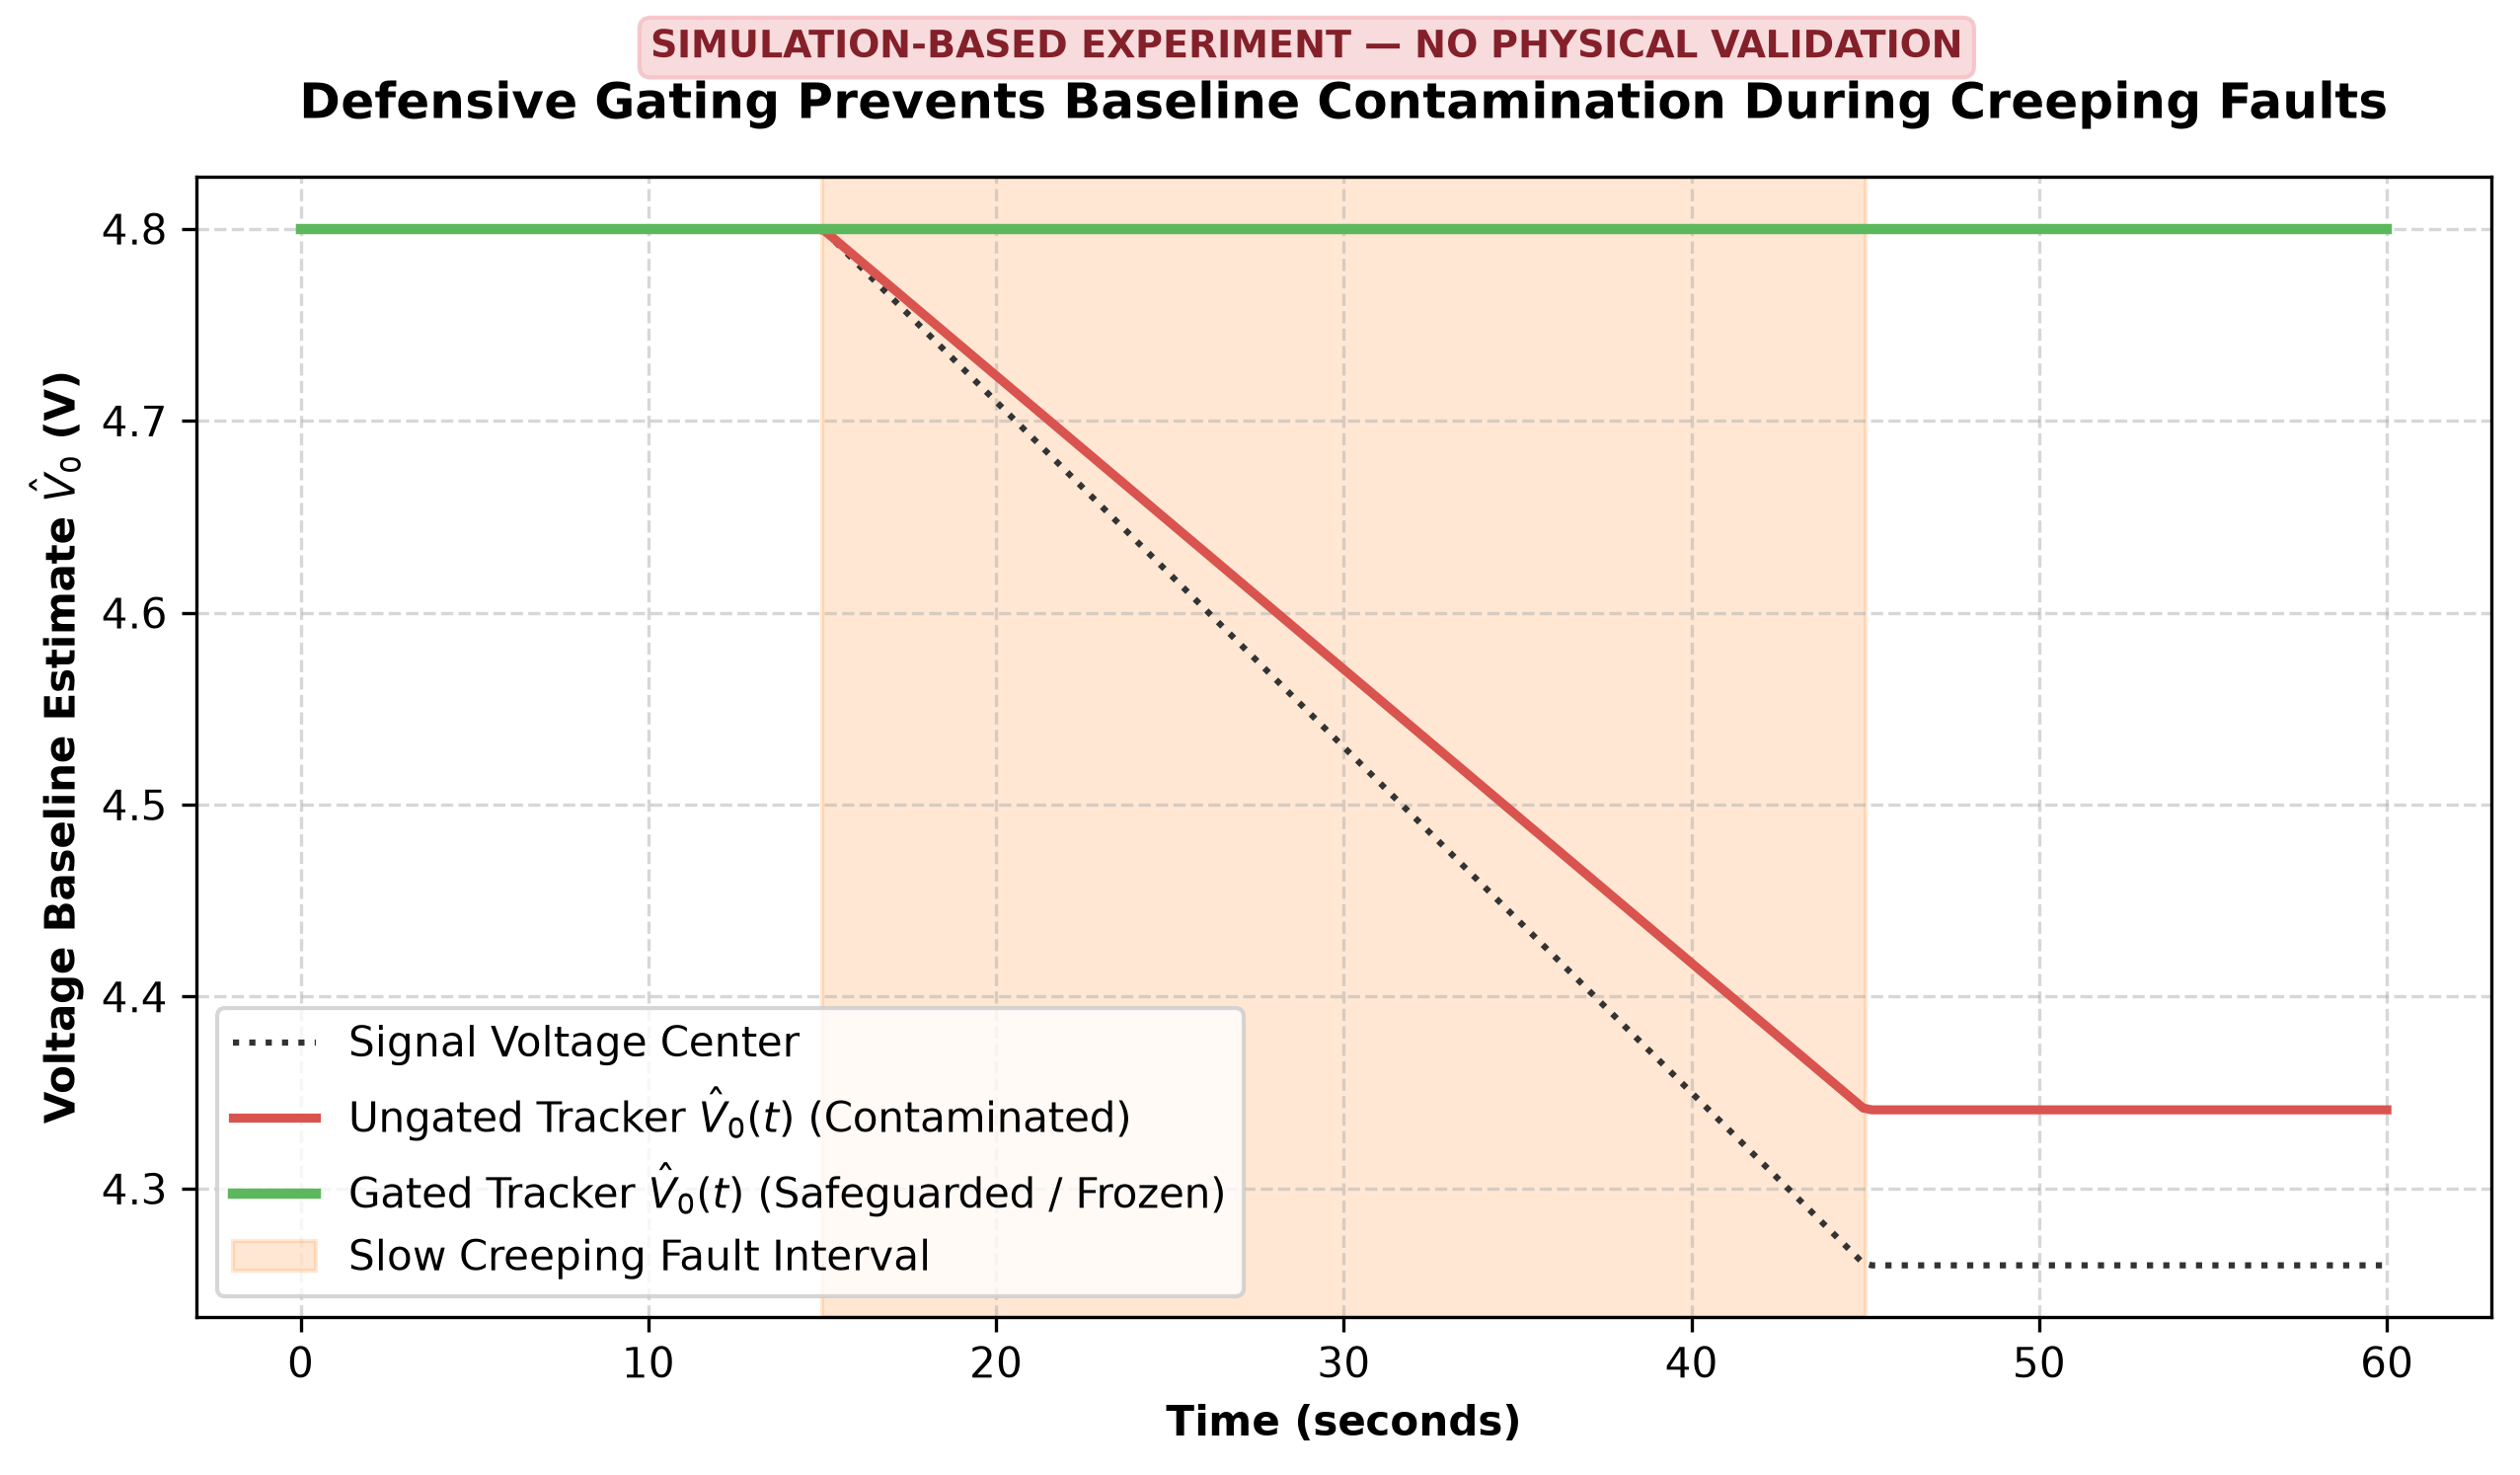
\includegraphics[width=0.92\columnwidth]{figures/fig5_contamination_prevention_trajectory.png}
\caption{Baseline voltage tracking trajectory during Scenario S9 (Slow Developing Fault). Ungated tracking adapts into the fault, shifting the baseline by 3.53\,mV (2.11\% contamination). Multi-stage defensive gating successfully freezes adaptation (0.00\% contamination).}
\label{fig:gating}
\end{figure}

\begin{table}[!t]
\caption{Adaptive Gating Ablation on Slow Creeping Fault (S9)}
\label{tab:gating}
\centering
\begingroup
\footnotesize
\setlength{\tabcolsep}{2.0pt}
\begin{tabular*}{\columnwidth}{@{\extracolsep{\fill}}lcccc@{}}
\toprule
\textbf{Gating Strategy} & \textbf{Contam.} & \textbf{Peak Shift} & \textbf{F1 (S9)} & \textbf{Bal. Acc.} \\
\midrule
Ungated Tracking          & 2.11\% & 3.53\,mV & 0.8920 & 0.9061 \\
No Confidence Gate        & 2.11\% & 3.53\,mV & 0.8912 & 0.9053 \\
No Stability Gate         & 0.00\% & 3.50\,mV & 0.8732 & 0.8877 \\
Fully Gated Adaptive (A3) & \textbf{0.00\%} & \textbf{3.50\,mV} & 0.8732 & 0.8877 \\
\bottomrule
\end{tabular*}
\endgroup
\end{table}

In ungated tracking, the tracker adapted during fault activity, resulting in a 2.11\% contamination rate and a 3.53\,mV baseline shift. Fully gated adaptive tracking (A3) achieved 0.00\% contamination. However, because the gates froze updates during fault development, the active baseline remained frozen at the initial reference value, explaining why M4 produced predictions identical to M3.

\begin{figure}[!t]
\centering
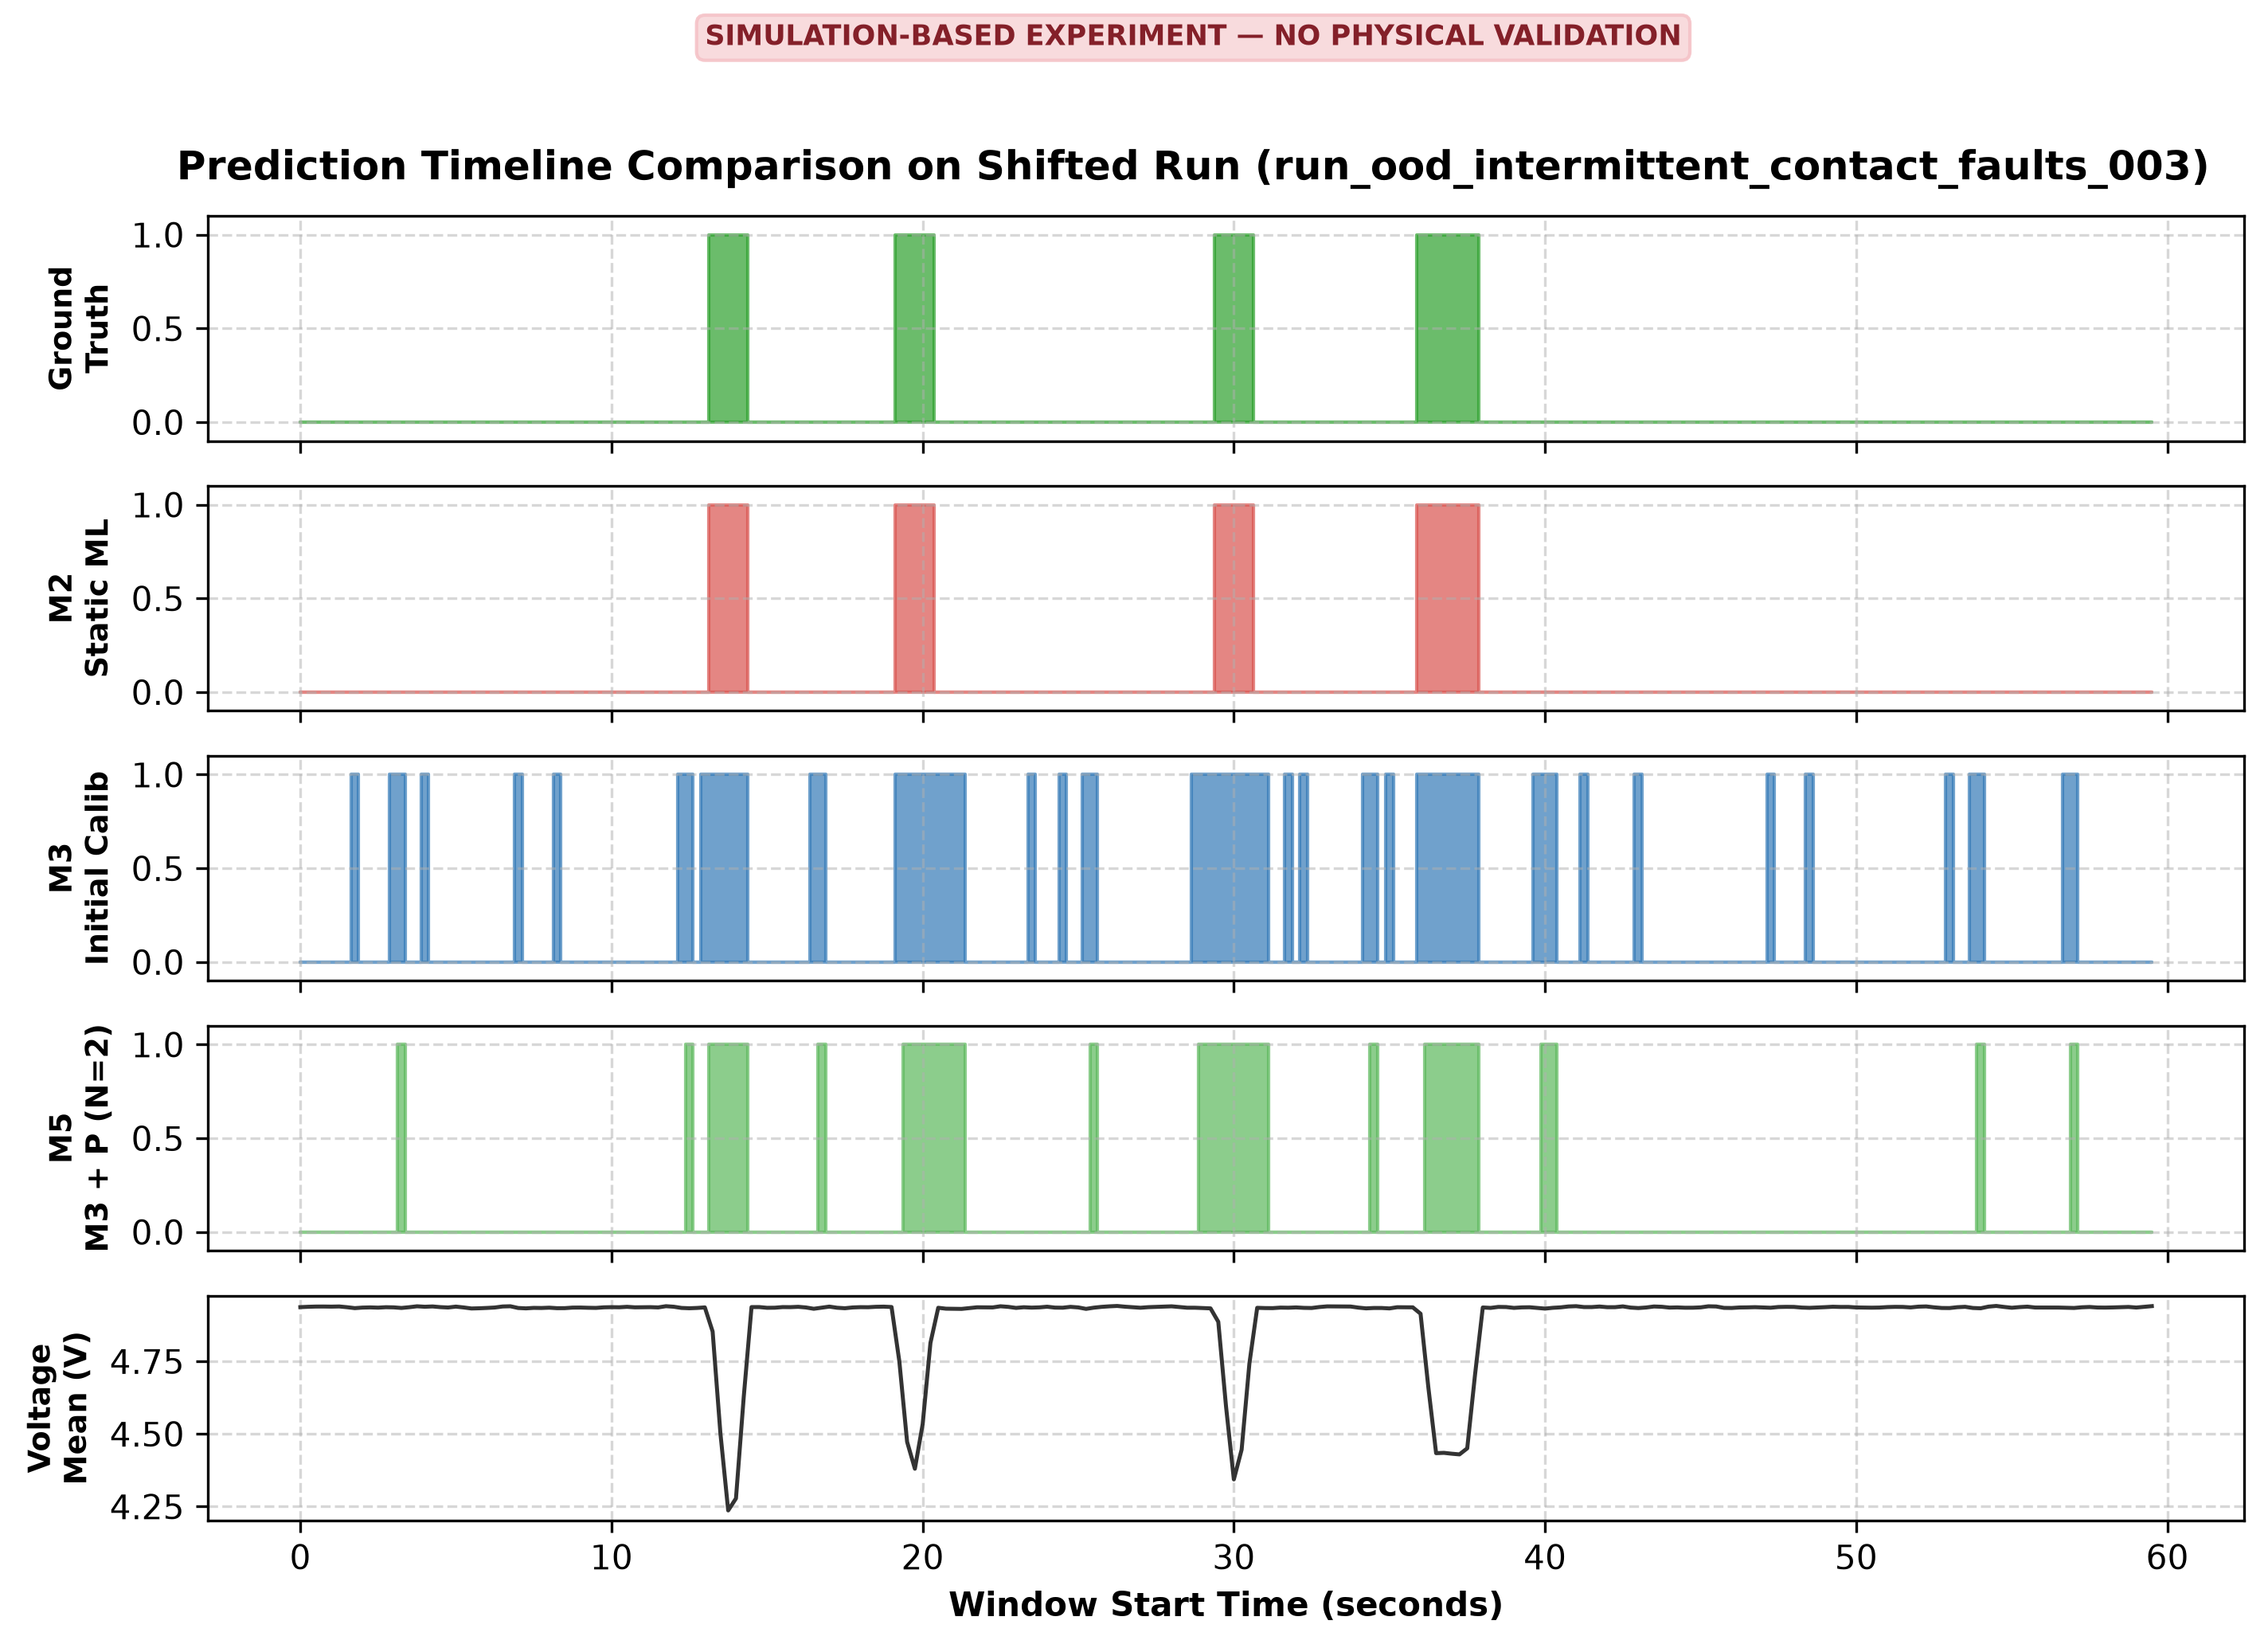
\includegraphics[width=0.92\columnwidth]{figures/fig6_prediction_timeline_overlay.png}
\caption{Prediction timeline overlay for a single representative simulation run comparing ground truth against M1, M2, M3, and M5. The overlay illustrates typical behavior on this individual run: M1 triggers false alarms during shifted conditions; M2 misses events under heavy load; M3 detects fault onsets with high sensitivity but produces transient noise spikes; M5 suppresses isolated spikes while tracking fault onsets. This trace illustrates individual sliding-window behavior on one run rather than uniform detection across all simulation runs.}
\label{fig:timeline}
\end{figure}

Representative detection timelines across methods are shown in Fig.~\ref{fig:timeline}, illustrating how M5 suppresses isolated single-window spikes during nominal operation while maintaining sharp detection responsiveness on fault onsets.

\subsection{Research Question Evaluation Scorecard}
Table~\ref{tab:scorecard} summarizes the definitive findings for the five research questions.

\begin{table*}[!t]
\caption{Research Questions Evaluation Scorecard}
\label{tab:scorecard}
\centering
\begingroup
\footnotesize
\setlength{\tabcolsep}{3.8pt}
\begin{tabularx}{\textwidth}{@{}l>{\raggedright\arraybackslash}X>{\raggedright\arraybackslash}p{4.2cm}>{\raggedright\arraybackslash}X@{}}
\toprule
\textbf{Research Question} & \textbf{Pre-Registered Hypothesis} & \textbf{Empirical Evidence (v5)} & \textbf{Scientific Verdict} \\
\midrule
\textbf{RQ1: Static ML} & Static ML trained on nominal telemetry fails under operational and sensor distribution shifts. & Static RF misses 23.44\% of OOD events (Event Recall = 76.56\%), collapses on S7 (Recall = 0.0000), and produces 860 FAs on S2 (Spec = 0.0000). & \textbf{Supported:} Static ML avoids fixed-threshold collapse but exhibits severe blind spots under load and resistance shifts. \\
\midrule
\textbf{RQ2: Reference Calib.} & A 5.0\,s initial reference calibration interval restores detection performance without continuous tracking. & Initial calibration (M3) restores Event Recall to 92.19\% (+15.63\% over M2) and BalAcc to 0.9028 ($\Delta\text{BalAcc} = +0.0896, p < 0.01$). & \textbf{Supported for Sensitivity:} Reference calibration successfully recovers obscured faults, though raw FAs require filtering. \\
\midrule
\textbf{RQ3: Adaptive Value} & Continuous confidence-gated adaptive calibration provides significant performance improvement over initial calibration. & Adaptive ML (M4) matches Initial Calibration (M3) identically: $\Delta\text{F1} = 0.0000$ (95\% CI $[0.0000, 0.0000]$, $p = 1.0000$). & \textbf{Refuted on OOD:} Continuous online adaptation provides zero measurable gain over a 5.0\,s initial reference baseline on the OOD partition ($\Delta\text{F1} = 0.0000, p = 1.0000$). \\
\midrule
\textbf{RQ4: Gating Integrity} & Multi-stage confidence and stability gating prevents tracker contamination during slow creeping faults. & Contamination rate drops from 2.11\% (ungated) to 0.00\% (M4/A3) on Scenario S9. & \textbf{Supported:} Defensive safety gates effectively prevent the baseline estimator from adapting into gradual fault resistance increases in this scenario. \\
\midrule
\textbf{RQ5: Persistence} & Causal multi-window persistence filtering suppresses transient false alarms at an acceptable detection latency cost. & Persistence $N=2$ (M5) cuts false alarms by 38.83\% ($515 \to 315$) and elevates F1 to 0.8559 ($p < 0.01$) at $+0.2085\,\text{s}$ latency. & \textbf{Supported:} Two-window persistence provides effective noise suppression (38.83\% fewer false-alarm events) while preserving all detected fault events. \\
\bottomrule
\end{tabularx}
\endgroup
\end{table*}

\section{Discussion}
The experimental results demonstrate that the combination of initial reference calibration and temporal persistence filtering offers a robust, computationally lightweight framework for power-path fault detection. 

\subsection{Why Initial Reference Calibration Works}
Static machine learning models fail under distribution shifts because they learn absolute decision boundaries on raw voltage and current levels. When the operating state changes (such as an increased steady-state charging current), terminal voltages drop naturally according to Ohm's law. A static classifier cannot determine whether a lower terminal voltage is caused by legitimate load current or an abnormal connector resistance. By subtracting the initial operating baseline ($\tilde{V} = V - \hat{V}_0$), reference calibration removes the operating point offset, enabling the classifier to evaluate relative fluctuations rather than absolute levels.

\subsection{Analysis of the Negative Adaptive Result}
A central finding of this research is that online adaptive calibration (M4) did not outperform static reference calibration (M3). This negative result is scientifically informative. In low-voltage power paths, physical faults such as contact oxidation occur on time scales that overlap with potential adaptive tracking rates. To prevent the estimator from absorbing creeping faults, defensive gates must be stringent. When gates are appropriately strict, they correctly freeze updates during abnormal behavior, leaving the baseline identical to the initial calibration. When gates are relaxed, the tracker contaminates. Consequently, for the evaluated scenarios, continuous online adaptation added algorithmic complexity without providing measurable detection benefit.

\subsection{Persistence Trade-Offs in Practical Systems}
While reference calibration restores fault sensitivity, it increases susceptibility to measurement noise, producing isolated single-window false alarms. The causal persistence filter effectively suppresses these false alarms because random Gaussian noise excursions rarely persist across multiple consecutive $0.25\,\text{s}$ strides. However, our ablation shows that persistence must be constrained: setting $N \ge 4$ introduces excessive latency ($> 0.70\,\text{s}$) and filters out short micro-interruptions.

\section{Limitations}
To maintain rigorous scientific standards, several explicit limitations must be stated:
\begin{enumerate}
    \item \textbf{Simulation-Only Study:} All findings are derived entirely from software simulation using an equivalent circuit. No physical USB-C cables, hardware test benches, or analog acquisition circuits were used.
    \item \textbf{Simplified Circuit Physics:} The simulator uses lumped-parameter resistance models. High-frequency RF transmission line effects, parasitic capacitances, contact arc physics, and thermal feedback are not modeled.
    \item \textbf{No Protocol Negotiation:} The model does not simulate USB Power Delivery (USB-PD) Configuration Channel (CC) communication, state-machine handshakes, or dynamic contract renegotiations (e.g., USB Type-C Release 2.2~\cite{usbtypec2022} and USB Power Delivery Revision 3.1 Version 1.7~\cite{usbpd2023}).
    \item \textbf{Known-Healthy Initialization:} The framework requires an initial $5.0\,\text{s}$ operating window that is guaranteed to be fault-free. If a system is initialized with an existing severe contact fault, the baseline will calibrate to the faulty state.
    \item \textbf{No Fault Localization:} Detections indicate anomalous path resistance but do not localize whether degradation originates in the receptacle, plug, cable wire, or solder joints.
    \item \textbf{Incomplete Detection and Residual False Alarms:} Method M5 achieved 92.19\% event recall (missing 5 of 64 events) and produced 7.92 false alarms per minute. It does not provide perfect detection.
\end{enumerate}

\section{Conclusion}
This study presented FlexPulse-ML, a simulation-based research framework evaluating reference-calibrated machine learning for intermittent fault detection in USB-C-inspired power paths. Through systematic experiments across ten controlled physical and operating scenarios, we demonstrated that conventional static machine learning classifiers degrade severely under distribution shift, missing nearly a quarter of fault events and failing entirely under load transitions. An initial five-second reference calibration interval substantially restores fault sensitivity, recovering event recall to 92.19\%. Combining initial calibration with a causal two-window persistence filter suppresses false-alarm events by 38.83\% and achieves an OOD F1-score of 0.8559 with an additional median detection latency of 0.2085\,seconds (total median delay 0.3407\,seconds). Furthermore, our evaluation confirmed that continuous online adaptation provided zero incremental benefit over initial reference calibration. Future work should transition these simulated architectures to physical experimental test benches to evaluate real-world noise distributions and hardware constraints.

\section*{Acknowledgment}
The author thanks the Department of Computer Science and Engineering at Presidency University, Bengaluru, for providing computing resources and academic guidance throughout this machine learning coursework project.

\bibliographystyle{IEEEtran}
\bibliography{references}

\end{document}
